\documentclass{article}
\usepackage{graphicx} % Required for inserting images
\usepackage{enumerate} %makes numbered lists
\usepackage{setspace}
\usepackage[hidelinks]{hyperref}
\usepackage{epsfig}  % for figures
\usepackage{url}  % Hyphenation of URLs.
\usepackage{lscape}  % Useful for wide tables or figures.
\usepackage[justification=raggedright]{caption}	% makes captions ragged right - thanks to Bryce Lobdell
\usepackage[labelfont=bf]{caption} % Makes the FIGURE X part of the figure caption bold
\usepackage{array} % For tables
\usepackage{multirow} %Merge multiple rows in tables
\usepackage{hhline} % for underlining table cells
\usepackage{framed} % frame around all subfigures
\usepackage{adjustbox} % custom frame around all subfigures
\usepackage{float}
\usepackage{booktabs}
\usepackage{amsmath}  % for math spacing
\usepackage{enumerate}
\usepackage{xcolor, soul} %lets us change the text color

\usepackage{geometry}
 \geometry{
 a4paper,
 total={170mm,257mm},
 left=20mm,
 top=20mm,
 }
\usepackage{textcomp}
\usepackage{tikz}
\usetikzlibrary{snakes,shapes,arrows,shapes.misc,shapes.arrows,positioning,decorations.markings,arrows.spaced,calc,decorations.text,arrows.meta,automata,intersections,patterns,intersections,through,backgrounds,external}

%\usetikzlibrary{external} %for Overleaf
%\tikzexternalize[prefix=tikz/] %for Overleaf
%\tikzexternalize[prefix=tikz/,optimize command away=\includepdf] %for Overleaf

\usepackage{pgfplots}
\pgfplotsset{compat=1.3} %<-- moves axis labels near ticklabels (respects tick label widths)
\usepgfplotslibrary{fillbetween}

% Define colors
\definecolor{Dorange}{RGB}{232,73,39}
\definecolor{Dlorange}{RGB}{227,165,52}
\definecolor{Ddblue}{RGB}{19,45,75}
\definecolor{Dlblue}{RGB}{1,111,185}
\definecolor{Dteal}{RGB}{39,207,249}
\definecolor{Mteal}{RGB}{169,236,253}
\definecolor{Lteal}{RGB}{212,245,254} 

%Commands to make the text red or blue
\newcommand{\red}[1]{\textcolor{red}{#1}}
\newcommand{\blue}[1]{\textcolor{blue}{#1}}
\newcommand{\teal}[1]{\textcolor{Dteal}{#1}}

\title{MechSE Web Reference Page - ME 200}
%\author{Updated}
\date

\begin{document}
\maketitle
\blue{Blue text:} Notes to whoever is transcribing these reference pages to the website

\red{Red text:} Unfinished secitons / questions

\teal{Teal text:} New content made by Alex
\tableofcontents
\newpage

\section{Thermodynamic Terminology and Definitions}
\subsection{System, boundaries and surroundings}
Energy and matter flow between a \textbf{thermodynamic system} and its \textbf{surroundings} that are separated by a \textbf{boundary}, lead to changes its internal state. An increase in its mass results when the matter flowing into the system is greater than that flowing out of the system. An increase in its internal energy results when the energy flowing into the system is greater than that flowing out of the system. When the flow rates into and out of the system are equal, the system is in a steady state. 

\begin{figure}[h]
\begin{center}
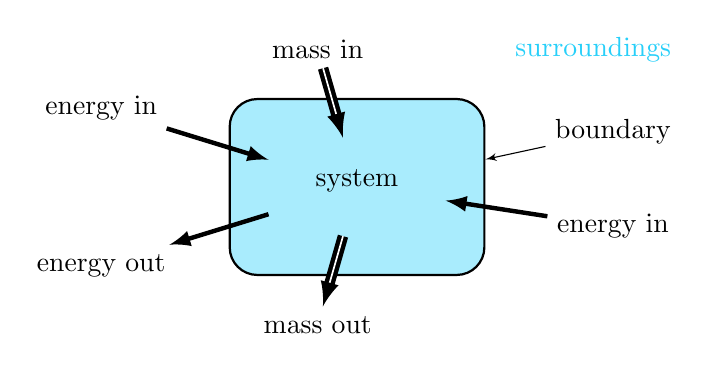
\begin{tikzpicture}[auto, node distance=1.75cm,>=latex']
	\node(1) [draw, fill=Mteal, rectangle, rounded corners=10pt, text width=3cm, text height = 1cm, text depth = 1cm, text centered,thick] {system};
	\node(100) [draw=none, fill=none, text width=2cm, text height=0.5cm, text depth=0.5cm]{};
	% Flow labels
	\node(2) [draw=none, fill=none, left of=1,yshift=1cm, xshift=-1.5cm]{energy in};
	\node(3) [draw=none, fill=none, left of=1,yshift=-1cm, xshift=-1.5cm]{energy out};
	\node(4) [draw=none, fill=none, above of=1,xshift=-0.5cm]{mass in};
	\node(5) [draw=none, fill=none, right of=1,yshift=-0.5cm, xshift=1.5cm]{energy in};
	\node(6) [draw=none, fill=none, right of=1,yshift = 0.7cm, xshift=1.5cm]{boundary};
	\node(7) [draw=none, fill=none, above of=1,xshift = 3cm]{\color{Dteal}surroundings};
	\node(8) [draw=none, fill=none, below of=1,xshift=-0.5cm]{mass out};
	% Flow arrows
	\draw [-latex, ultra thick] (2) -- (100);
	\draw [-latex,double, ultra thick] (4) -- (100);
	\draw [-latex, ultra thick] (100) -- (3);
	\draw [-latex,  ultra thick] (5) -- (100);
	\draw [->] (6) -- (1);
	\draw [-latex, double,  ultra thick] (100) -- (8);
\end{tikzpicture}
\end{center}
\caption{A schematic representation of a thermodynamic system illustrating its key features including depictions of energy and mass flows.}\label{fig:SysSchematic}
\end{figure}
%%%%%%%%%%%%%%%%%%%%%%%%%%%%%%%%%%%%%%%%%%%%%%%
%%%%%%%%%%%%%%%%%%%%%%%%%%%%%%%%%%%%%%%%%%%%%%%
\paragraph{Steady-state:} When the flow rates into and out of the system are equal, the system is in a \textbf{steady state}
\paragraph{Transient:} The state of a thermodynamic system is \textbf{transient} if it is not in steady state.

\subsubsection{Types of Systems: Closed, Open, and Isolated Systems} 
\paragraph{Closed System:} Mass cannot flow in or out of the system, therefore energy is transferred via only heat or work.

\paragraph{Open System:} An open system can exchange both energy and matter with its surroundings.

\paragraph{Isolated System:} A system is isolated from its environment, meaning neither matter nor energy may flow in or out of the system. 
%%%%%%%%%%%%%%%%%%%%%%%%%%%%%%%%%%%%%%%%%%%%%%%
%%%%%%%%%%%%%%%%%%%%%%%%%%%%%%%%%%%%%%%%%%%%%%%
\subsection{Units of Interest}
\subsubsection{Typical Units in SI and English Systems}

\begin{table*}[h]
\small
  \caption{\ Typical Units in SI and English Systems: Dimensions}
  \label{tbl:units}
  \begin{tabular*}{\textwidth}{@{\extracolsep{\fill}}lllllll}
    \hline
    Dimension & SI Units  & English Engineering Unit \\
    \hline
    Force & newton (N) &  pound force (lbf) \\
    Length & meter (m) &  foot (ft) \\
    Mass & kilogram (kg) &  pound mass (lb) \\
    Time & second (s) &  second (s) \\
  \end{tabular*}
\end{table*}

\begin{table*}[h]
\small
  \caption{\ Typical Units in SI and English Systems: State properties}
  \label{tbl:units}
  \begin{tabular*}{\textwidth}{@{\extracolsep{\fill}}lllllll}
    \hline
    State property & SI Units  & English Engineering Unit \\
    \hline
    Pressure & Pascals (Pa) &  Pound Force per square inch (psi) \\
      & 1 Pa = N/m$^2$ = J/m$^3$ &  \\
    Volume & m$^3$ &  ft$^3$ \\
    Temperature & degrees Celcius ($^{\circ}$C) &  degrees Fahrenheit ($^{\circ}$F) \\
    Absolute Temperature & Kelvin (K) &  degree Rankine ($^{\circ}$R) \\
    Internal Energy, Enthalpy & Joules (J) &  British thermal Unit (Btu) \\
     & Newton-meter (N$\cdot$m) & Foot-pound force (ft$\cdot$lbf)\\
    Entropy  &  (J/K) & Btu/$^{\circ}$R \\
  \end{tabular*}
\end{table*}
\subsubsection{Useful Conversions}
\paragraph{Pressure}
\begin{align*}
  1~\textrm{standard atm} = 1.01325 ~\textrm{bar} = 1.01325 \times 10^{5} ~\textrm{Pa} = 14.696~\textrm{psi} = 760~\textrm{mmHg} = 29.92~\textrm{inHg}  
\end{align*}

\paragraph{Temperature}
\begin{align*}
    \textrm{Fahrenheit to Rankine:}~ ^{\circ}\textrm{R} = ^{\circ}\textrm{F} + 459.67\\
    \textrm{Celsius to Kelvin:}~ \textrm{K} = ^{\circ}\textrm{C} + 273.15
\end{align*}
\paragraph{Energy}
\begin{align*}
    \textrm{Btu to ft$\cdot$lbf:}~ 1~\textrm{Btu} = 778.18~ \textrm{ft}\cdot\textrm{lbf}
\end{align*}
\subsubsection{Useful Constants}
\paragraph{Gravity}
\begin{align*}
    9.8~\textrm{N} = 1~\textrm{kg}\times 9.8~ \textrm{m}/\textrm{s}^2 \\
    1~\textrm{lbf} = 1~\textrm{lb}\times 32~ \textrm{ft}/\textrm{s}^2
\end{align*}
\paragraph{Universal Gas Constant, $\overline{R}$}
\begin{align*}
    \overline {R} = 8.314~\textrm{kJ/kmol}\cdot \textrm{K} \\
    \overline {R} = 1545~\textrm{ft}\cdot \textrm{lbf}/\textrm{lbmol}\cdot ^{\circ}\textrm{R} \\
    \overline {R} = 1.986~\textrm{Btu}/\textrm{lbmol}\cdot ^{\circ}\textrm{R} 
\end{align*}
\paragraph{Molecular weights $M$ of common substances (1 g/mol = 1 kg/kmol = 1 lb/lbmol): $R= \frac{\overline{R}}{M}$}
\begin{itemize}
    \item Air- 28.97 g/mol
    \item Carbon dioxide CO$_2$- 44.01 g/mol
    \item Ethane C$_2$H$_6$- 30.07 g/mol
    \item Hydrogen H$_2$- 2.01 g/mol
    \item Methane CH$_4$- 16.04 g/mol
    \item Nitrogen N$_2$- 28.01 g/mol
    \item Oxygen O$_2$- 32.00 g/mol
    \item Refrigerant 22- 86.48 g/mol
    \item Refrigerant 134a- 102.3 g/mol
    \item Water H$_2$O- 18.015 g/mol
\end{itemize}
\subsubsection{Helpful Math Expressions}
\paragraph{Integrals:}
\begin{equation*}
    \int_{y_a}^{y_b} \frac{1}{y}dy = ln(y)|_{y_a}^{y_b}
\end{equation*}
\begin{equation*}
    \int_{y_a}^{y_b} \frac{1}{y^{\gamma}}dy = - \left \frac{1}{\gamma -1}\frac{1}{y^{\gamma -1}}\right |_{y_a}^{y_b} ,~\textrm{for}~\gamma \neq 1
\end{equation*}
\paragraph{Natural Logs:}
\begin{equation*}
    ln(ab)= ln(a)+ln(b)
\end{equation*}
\begin{equation*}
    e^{aln(b)} = b^a
\end{equation*}
%%%%%%%%%%%%%%%%%%%%%%%%%%%%%%%%%%%%%%%%%%%%%%%
%%%%%%%%%%%%%%%%%%%%%%%%%%%%%%%%%%%%%%%%%%%%%%%
\subsection{Mass and Mass Flow}
As matter flows in and out of a thermodynamic system, the amount of mass in the system at time $t$ by is defined by $m(t)$, then 
\begin{equation}\label{eq:MassBalanceDiff}
\frac{dm}{dt}(t) = \sum_{in}\dot{m}_{in}(t) - \sum_{out}\dot{m}_{out}(t),
\end{equation}
refers to `the rate of change of the mass of the system.' The sums on the right add up all mass flows into and out of the system, respectively. If this quantity is positive, then the mass of the system is increasing. If it is negative, the mass of the system must be decreasing, as long as there is still mass left inside the system. 

If these flow rates are known functions of time, then this equation implies that
\begin{equation}\label{eq:MassBalanceInt}
m(t) = m(0) + \int_0^t \left( \sum_{in}\dot{m}_{in}(\tau) - \sum_{out}\dot{m}_{out}(\tau)\right) d\tau,
\end{equation}
where $m(0)$ is the initial value of the mass in the system at time $t=0$. Integrating Eqn.~\eqref{eq:MassBalanceInt} with respect to time yields.
\begin{equation}\label{eq:MassBalanceInt2}
m(t) - m(0) = \Delta m =  \sum_{in}m_{in}- \sum_{out}m_{out}
\end{equation}
where $m_{in}$ and $m_{out}$ are the total quantities of mass transferred in or out of the system for a given set of processes. 
\begin{figure}[h]
\begin{center}
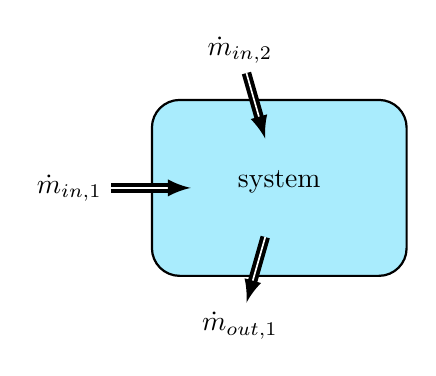
\begin{tikzpicture}[auto, node distance=1.75cm,>=latex']
	\node(1) [draw, fill=Mteal, rectangle, rounded corners=10pt, text width=3cm, text height = 1cm, text depth = 1cm, text centered,thick] {system};
	\node(100) [draw=none, fill=none, text width=2cm, text height=0.5cm, text depth=0.5cm]{};
	% Flow labels
	\node(2) [draw=none, fill=none, left=0.5cm of 1.west]{$\dot{m}_{in,1}$};
	\node(3) [draw=none, fill=none, above of=1,xshift=-0.5cm]{$\dot{m}_{in,2}$};
	\node(4) [draw=none, fill=none, below of=1,xshift=-0.5cm]{$\dot{m}_{out,1}$};
	% Flow arrows
	\draw [-latex,double,line width=0.5mm] (2) -- (100);
	\draw [-latex,double,line width=0.5mm] (3) -- (100);
	\draw [-latex,double,line width=0.5mm] (100) -- (4);
\end{tikzpicture}
\end{center}
\caption{A system whose state is changing due to mass flow.}\label{fig:SysSchematic}
\end{figure}

Given the thermodynamic system shown in Figure \ref{fig:SysSchematic}, one can write the rate of change of mass of the system equals the following quantity,
\begin{equation}
\dot{m}_{in,1} +\dot{m}_{in,2} - \dot{m}_{out,1}
\end{equation}
%%%%%%%%%%%%%%%%%%%%%%%%%%%%%%%%%%%%%%%%%%%%%%%%
%%%%%%%%%%%%%%%%%%%%%%%%%%%%%%%%%%%%%%%%%%%%%%%%
\subsection{\teal{Volume and Volume Flow}}
The volume $V$ of a system is an extensive parameter for describing its thermodynamic state. The specific volume $v$, an intensive property, is the system's volume per unit mass. Volume is a function of state and is interdependent with other thermodynamic properties such as pressure and temperature. 
\paragraph{Specific Volume}
Specific volume is the volume per unit mass
\begin{equation*}
    v=\frac{V}{m}={\frac{\textrm{m}^3}{\textrm{kg}}}
\end{equation*}
\subsubsection{Volume Flow}
As mass flows into a system, energy increases by the addition of both the internal energy of the additional mass \emph{and} the $pV$ work done by the volume occupied by the mass on the system as it enters, and vice versa.
%%%%%%%%%%%%%%%%%%%%%%%%%%%%%%%%%%%%%%%%%%%%%%%%%%%%%%%%%%%%%%%%%%%%%%%%%%%%%%%%%%%%%%%%%%%%%%%%%%%%%%%%%%%%%%%%%%%%%%%%%%%%%%%%
\begin{figure}[h]
\begin{center}
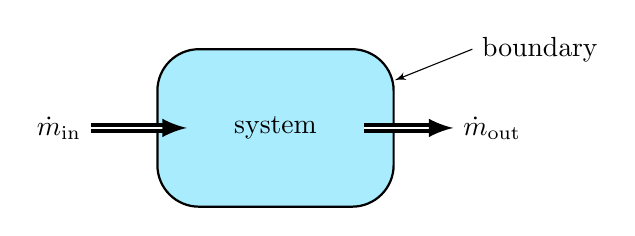
\begin{tikzpicture}[auto, node distance=1.75cm,>=latex']
	\node(1) [draw, fill=Mteal, rectangle, rounded corners=15pt, minimum width=3cm, minimum height = 2cm, text centered,thick] {system};
	\node(100) [draw=none, fill=none, text width=2cm, text height=0.5cm, text depth=0.5cm]{};
	% Flow labels
	\node(2) [draw=none, fill=none, left of=1,xshift=-1cm]{$\dot{m}_{\text{in}}$};
	\node(4) [draw=none, fill=none, right of=1,xshift=1cm]{$\dot{m}_{\text{out}}$};
	% Flow arrows
	\draw [-latex, double, ultra thick] (2) -- (100);
	\draw[-latex,double, ultra thick] (100) -- (4);t
	\draw[->] ($ (1) + (2.5,1)$) node[right]{boundary} -- (1);
\end{tikzpicture}
\end{center}
\end{figure}
%%%%%%%%%%%%%%%%%%%%%%%%%%%%%%%%%%%%%%%%%%%%%%%%%%%%%%%%%%%%%%%%%%%%%%%%%%%%%%%%%%%%%%%%%%%%%%%%%%%%%%%%%%%%%%%%%%%%%%%%%%%%%%%%
\begin{figure}
\begin{center}
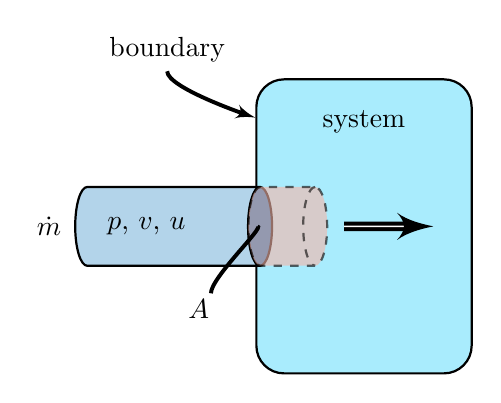
\begin{tikzpicture}[auto, node distance=1.75cm,>=latex']
	\node(1) [draw, fill=Mteal, rectangle, rounded corners=10pt, text width=2.5cm, text height = 0.5cm, text depth = 3cm, text centered,thick] {system};
	\node(100) [draw=none, fill=none, text width=2cm, text height=0.5cm, text depth=0.5cm]{};
	\node (2) [cylinder,thick,aspect=1.3,cylinder uses custom fill, cylinder body fill=Dlblue!30,cylinder end fill=Dlblue,shape border rotate=0, draw,minimum height=2.5cm,
	minimum width=1cm,xshift=-0.8cm,left of=1] { };
	\node(200) [draw=none, fill=none, right=0.3cm of 2.west]{$p$, $v$, $u$};
	\node (3) [cylinder,thick,aspect=1.3, fill=Dorange!40,opacity=0.6, dashed,shape border rotate=0, draw,minimum height=1cm,minimum width=1cm,left of=1,xshift=0.65cm]{};
	% Flow labels
	\node(201) [draw=none, fill=none, left of=2, xshift=0.3cm]{$\dot{m}$};
	\node(301) [draw=none, fill=none, below of=3, xshift=-1.0cm, yshift=0.7cm]{$A$};
	\node(101) [draw=none, fill=none, above of=1, xshift=-2.5cm, yshift=0.5cm]{boundary};
	% Flow arrows
	\draw [double,->, line width=0.5mm] ([xshift=0.2cm]3.east) -- ([xshift=-0.5cm]1.east);
	\draw [->, line width=0.5mm] (101) .. controls +(down:0.5cm) and +(left:0cm) .. ([yshift=-0.5cm]1.north west);
	\draw [-, line width=0.5mm] ([yshift=0.2cm,xshift=-0.1cm]301.east) .. controls +(up:0.2cm) and +(right:0.1cm) .. ([xshift=-0.2cm]2.east);
\end{tikzpicture}
\end{center}
\end{figure}
%%%%%%%%%%%%%%%%%%%%%%%%%%%%%%%%%%%%%%%%%%%%%%%%%%%%%%%%%%%%%%%%%%%%%%%%%%%%%%%%%%%%%%%%%%%%%%%%%%%%%%%%%%%%%%%%%%%%%%%%%%%%%%%%

A mass flow having rate $\dot{m}$ with cross-sectional area, $A$, \underline{slowly} enters a system. The mass is at a pressure $p$, has a specific volume $v$, and has a specific internal energy, $u$, relative to some reference state.
The mass flows into the system, over a given time interval $\Delta t$, increasing the internal energy of the system as it enters, by:
\begin{equation}
\label{eqn:Deltau_dotm}
\dot{m}\Delta t u=mu.
\end{equation}

The volume occupied by the portion of the stream entering a system is defined by,
\begin{equation}
V_{\text{in-flow}}=\dot{m}\Delta t v=mv
\end{equation}
This volume is pushed at constant pressure, $p$, into the system, is doing $pV$ work on the system, which will be described further in \blue{section \ref{sec:pvwork}. (link this to section)}

%%%%%%%%%%%%%%%%%%%%%%%%%%%%%%%%%%%%%%%%%%%%%%%%
%%%%%%%%%%%%%%%%%%%%%%%%%%%%%%%%%%%%%%%%%%%%%%%%
\subsection{Energy and Energy Flow}
\subsubsection{Internal Energy}
The \textbf{internal energy}, $U$, of a thermodynamic system relative to some \textbf{reference state} $U_0$ is the energy required to set up the positions and motions of the atoms and molecules within the system from their positions and motions in the reference state. When the system is in its reference state, its relative internal energy equals $0$. 
\begin{equation}\label{eq:Ebalance}
\Delta U = U - U_0 = \textrm{energy}_{in} - \textrm{energy}_{out}
\end{equation}
\vspace{12pt}

The addition of energy to a system in its reference state will result in the system having a positive relative internal energy. The removal of energy from a system in its reference state will result in the system having a negative relative internal energy. Eqn.~\eqref{eq:MassBalanceInt2}.

\begin{figure}[h]
\begin{center}
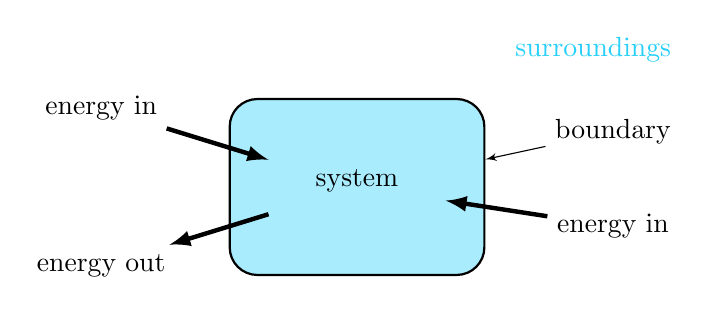
\begin{tikzpicture}[auto, node distance=1.75cm,>=latex']
	\node(1) [draw, fill=Mteal, rectangle, rounded corners=10pt, text width=3cm, text height = 1cm, text depth = 1cm, text centered,thick] {system};
	\node(100) [draw=none, fill=none, text width=2cm, text height=0.5cm, text depth=0.5cm]{};
	% Flow labels
	\node(2) [draw=none, fill=none, left of=1,yshift=1cm, xshift=-1.5cm]{energy in};
	\node(3) [draw=none, fill=none, left of=1,yshift=-1cm, xshift=-1.5cm]{energy out};
	\node(4) [draw=none, fill=none, right of=1,yshift=-0.5cm, xshift=1.5cm]{energy in};
	\node(5) [draw=none, fill=none, right of=1,yshift = 0.7cm, xshift=1.5cm]{boundary};
	\node(6) [draw=none, fill=none, above of=1,xshift = 3cm]{\color{Dteal}surroundings};
	% Flow arrows
	\draw [-latex, ultra thick] (2) -- (100);
	\draw [-latex, ultra thick] (100) -- (3);
	\draw [-latex,  ultra thick] (4) -- (100);
	\draw [->] (5) -- (1);
\end{tikzpicture}
\end{center}
\caption{A schematic representation of a thermodynamic system illustrating energy flows.}\label{fig:SysSchematic}
\end{figure}

\paragraph{Internal Energy Contributions} The internal energy ($U$) of a system is affected by the energetic contributions from heat flow ($Q$) in and out of a system and work ($W$) done by or on a system.  
\begin{equation}\label{eq:Ebal}
\Delta U = Q -  W.
\end{equation}
\paragraph{Sign Convention:} These energetic changes affect thermodynamic systems as follows:
\begin{enumerate}
    \item When heat is transferred to the system, the system energy increases (positive heat transfer).
    \item When the system does work on its surroundings, the system energy decreases (negative sign in front of work done by system).
    \item When the system transfers heat to the surroundings, the system energy decreases (negative heat transfer).
    \item When work is done on to the system, the system energy increases (positive sign in front of work done on system).
    
\end{enumerate}

\begin{figure}[h]
\begin{center}
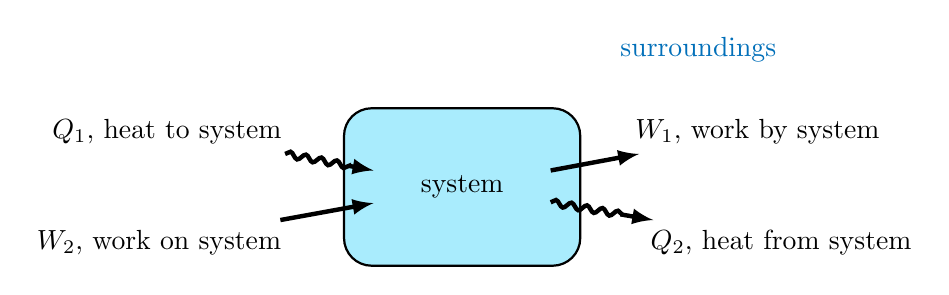
\begin{tikzpicture}[auto, node distance=1.75cm,>=latex']
	\node(1) [draw, fill=Mteal, rectangle, rounded corners=10pt, minimum width=3cm, minimum height = 2cm, text centered,thick] {system};
	\node(100) [draw=none, fill=none, text width=2cm, text height=0.5cm, text depth=0.5cm]{};
	% Flow labels
	\node(2) [draw=none, fill=none, left of=1,yshift=0.7cm, xshift=-2cm]{$Q_{1}$, heat to system};
	\node(3) [draw=none, fill=none, left of=1,yshift=-0.7cm, xshift=-2.1cm]{$W_{2}$, work on system};
	\node(4) [draw=none, fill=none, right of=1,yshift=-0.7cm, xshift=2.3cm]{$Q_{2}$, heat from system};
	\node(5) [draw=none, fill=none, right of=1,yshift=0.7cm, xshift=2cm]{$W_{1}$, work by system};
	\node(6) [draw=none, fill=none, above of=1,xshift = 3cm]{\color{Dlblue}surroundings};
	% Flow arrows
	\draw [-latex,decorate,decoration={snake,amplitude=.4mm,segment length=2mm, post length=9pt}, ultra thick] (2) -- (100);
	\draw[-latex,decorate,decoration={snake,amplitude=.4mm,segment length=2mm ,post length=9pt}, ultra thick] (100) -- (4);
	\draw [-latex, ultra thick] (3) -- (100);
	\draw [-latex, ultra thick] (100) -- (5);
\end{tikzpicture}
\end{center}
\caption{A schematic illustrating the direction of energy flow when heat is transferred to/from the system and work is performed on or by the system.}\label{fig:SysSchematic1}	
\end{figure}

Given the system shown in Figure \ref{fig:SysSchematic1}, the net work done by the system is $W_1-W_2$. The net heat transferred to the system is $Q_1-Q_2$. The change in system energy is
\begin{equation}
\Delta U = Q_1-Q_2-(W_1-W_2).
\end{equation}
%%%%%%%%%%%%%%%%%%%%%%%%%%%%%%%%%%%%%%%%%%%%%%%%%%%%%%%%%%%%%%%%%%%%%%%%%%%%%%%%%%%%%%%%%%%%%%%%%%%%%%%%%%%%%%%%%%%%%%%%%%%%%%%%%%
\subsubsection{Potential Energy}
A system may find itself subject to a conservative force in a position that differs from a reference position.  In this scenario, work has been done against a conservative force, such as changing the height, $h$, to change the potential energy.
%%%%%%%%%%%%%%%%%%%%%%%%%%%%%%%%%%%%%%%%%%%%%%%%%%%%%%%%%%%%%%%%%%%%%%%%%%%%%%%%%%%%%%%%%%%%%%%%%%%%%%%%%%%%%%%%%%%%%%%%%%%%%%%%%%

\begin{figure}[h]
\begin{center}
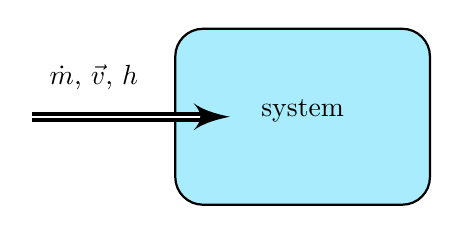
\begin{tikzpicture}[auto, node distance=1.75cm,>=latex']
	\node(1) [draw, fill=Mteal, rectangle, rounded corners=10pt, text width=3cm, text height = 1cm, text depth = 1cm, text centered,thick] {system};
	\node(100) [draw=none, fill=none, text width=2cm, text height=0.5cm, text depth=0.5cm]{};
	% Flow labels
	\node(2) [draw=none, fill=none, left of=1,yshift=0.5cm, xshift=-0.9cm]{$\dot{m}$, $\vec{v}$, $h$};
	% Flow arrows
	\draw [double,->, line width=0.5mm] ([xshift=-1.8cm]1.west) -- ([xshift=0.2cm]100.west);
\end{tikzpicture}
\end{center}
\end{figure}
%%%%%%%%%%%%%%%%%%%%%%%%%%%%%%%%%%%%%%%%%%%%%%%%%%%%%%%%%%%%%%%%%%%%%%%%%%%%%%%%%%%%%%%%%%%%%%%%%%%%%%%%%%%%%%%%%%%%%%%%%%%%%%%%%%
\noindent Typical conservative forces include elastic potential energy, \emph{e.g.}, a spring, and electric potential energy. For the particular case of gravity,
\begin{equation}\label{eq:PE}
\begin{split}
W_{\text{PE}_g}&=\int_{z_1}^{z_2}mg\,dz\\
&=mg(z_2-z_1)
\end{split}
\end{equation}
Thus the change in the gravitational potential energy of the system.
\begin{equation}
    W_{\text{PE}_g}=\Delta \text{PE}_g 
\end{equation}
%%%%%%%%%%%%%%%%%%%%%%%%%%%%%%%%%%%%%%%%%%%%%%%%%%%%%%%%%%%%%%%%%%%%%%%%%%%%%%%%%%%%%%%%%%%%%%%%%%%%%%%%%%%%%%%%%%%%%%%%%%%%%%%%%%


\subsubsection{Kinetic Energy}
A system may find itself in motion with respect to a reference frame. In this first case, work has been done to
accelerate the system to its velocity. Work done is defined by forces acting over a distance, and work $W_{\text{KE}}$ can be done to accelerate the system to its velocity,
\begin{equation}
W_{\text{KE}}=\int_{\vec{x_1}}^{\vec{x_2}}\vec{f}\,d\vec{x}.
\end{equation}
Force is determined from Newton's 2nd law:
\begin{equation}
\vec{f}=m\frac{d\vec{v}}{dt}=m\frac{d\vec{v}}{d\vec{x}}\underbrace{\frac{d\vec{x}}{dt}}_{\vec{v}}=m\vec{v}\frac{d\vec{v}}{d\vec{x}}
\end{equation}
This results in the following relationship for work done via kinetic energy change ($W_{\text{KE}}$)
\begin{equation}\label{eq:KE}
\begin{split}
W_{\text{KE}}&=\int_{\vec{v_1}}^{\vec{v_2}}m\vec{v}\,d\vec{v}\\
&=\frac{1}{2}m(\vec{v}_2^2-\vec{v}_1^1).
\end{split}
\end{equation}
Thus the change in kinetic energy of the system.
\begin{equation}
    W_{\text{KE}}=\Delta \text{KE}
\end{equation}

\subsubsection{Enthalpy}
Enthalpy is a state function that is the sum of a system's internal energy $\mu$ and the product of its pressure and volume $pv$.
\paragraph{Relative Specific Enthalpy}
The sum $u+pv$ appears frequently in thermodynamic discussion so it is conveniently defined as relative specific enthalpy $h$, consisting of the same atomic and molecular kinetic and potential energies as specific internal energy $u$, but with the addition of \emph{flow work}, $pv$
\begin{equation}
\label{eqn:RelativeEnthalpy}
h=u+pv.
\end{equation}
%%%%%%%%%%%%%%%%%%%%%%%%%%%%%%%%%%%%%%%%%%%%%%%%%%%%%%%%%%%%%%%%%%%%%%%%%%%%%%%%%%%%%%%%%%%%%%%%%%%%%%%%%%%%%%%%%%%%%%%%%%%%%%%%%%
\subsection{\blue{Entropy}}
\blue{We would like this to link to the Entropy page :)}

\section{Substances}
\subsection{\teal{Phases of matter}} %missing title
A phase of matter is homogeneous in both its molecular composition and the structure of its molecules with respect to one another. 

\paragraph{Pure Substance:} A pure substance is when a substance occurs in a single phase and is composed of a single type of molecule. 
\teal{\paragraph{Solid:} A substance that has a definite shape and volume is a solid.  The molecules in a solid are tightly packed, and cannot move past one another but vibrate.}
\teal{\paragraph{Liquid:} A substance that has a definite volume, but no definite shape is a liquid, taking on the shape of their container.  The molecules in a liquid are constantly moving yet still in contact with one another.}
\teal{\paragraph{Gas:} A substance with no definite shape or volume, gases take on the shape or volume of the container they are surrounded by.  Molecules can move freely and have negligible intermolecular interactions.}

\subsubsection{Phase Diagrams}
A phase diagram is like a map and predicts the phase of a substance according to its thermodynamic properties: $p$, $T$, $v$, $u$, and $h$. An example of a $pv$ liquid-vapor phase diagram for a pure substance is shown below:
\begin{figure}[h]
\begin{center}
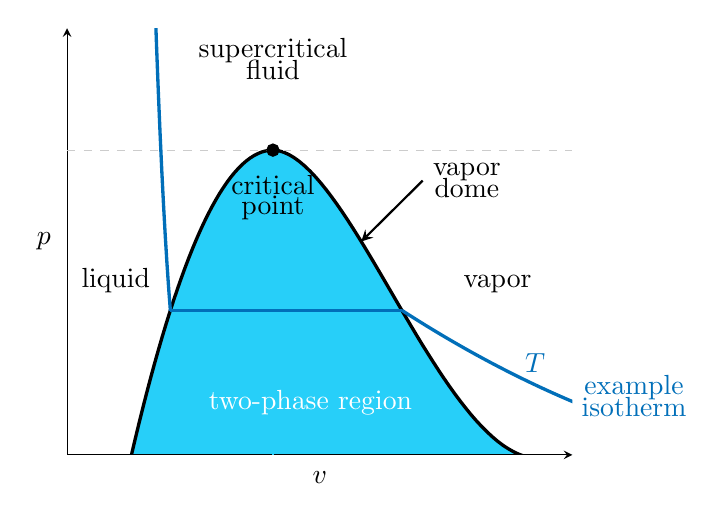
\begin{tikzpicture}[auto,every text node part/.style={align=center},
	declare function={
        		curveL(\x) = -0.7*\x^2+10;
		curveR(\x) = -1*\x^2 + 0.3*x^2.5 + 10;
		TcurveL(\x) = 2*(\x+1.5)^4;
		TcurveR(\x) = -1*x+7.83+0.03*x^2;
  	}
	]
	
% left plot
	\node (ref) at (0,0) [draw=none, coordinate] {};
	\begin{axis} [at={(ref)},xmin=-5.5, ymin=0, xmax=8, ymax = 14, samples = 50, 
			ytick=\empty, yticklabels={}, ylabel style={rotate=-90},
			xtick=\empty, xticklabels={},
			ylabel={$p$}, xlabel={$v$},
			width = 8cm, height=7cm, axis y line = left, axis x line = bottom,
			thick, fill between/on layer={axis background}]
		%L+V dome
		\addplot[very thick,domain=-5:0, name path=L] {curveL(x)};	
		\path[name path=axL] (axis cs:-5, 0) -- (axis cs:0, 0);	
		\addplot[very thick,domain=0:7, name path=R] {curveR(x)};
		\path[name path=axR] (axis cs:0, 0) -- (axis cs:14, 0);
		\addplot [fill=Dteal]
		fill between [
			of = L and axL,
			soft clip={domain=-5:0},
		];
		\addplot [fill=Dteal]
		fill between [
			of = R and axR,
			soft clip={domain=0:14},
		];
				\addplot[color=Dteal] coordinates {(0,10) (0,0)}; % cover seam	
	
		%critical point
		\addplot[mark=*] coordinates {(0,10)};
		\addplot[dashed,thin,domain=-5.5:8,color=black!20] {10};
		
		
		% isotherm 
		\addplot[very thick,domain=-5:-2.74, Dlblue] {TcurveL(x)};	
		\addplot[very thick,domain=-2.74:3.4445,Dlblue] {4.74142};
		\addplot[very thick,domain=3.44449:14, Dlblue] {TcurveR(x)};	
		

		
		\node [below, color=black, yshift=-0.2cm] at (axis cs:0, 10) {critical \\[-5pt] point};
		\node [above, color=black] at (axis cs:6, 5) {vapor};
		\node [above, color=black] at (axis cs:-4.2, 5) {liquid};
		\node [color=Dlblue] at (axis cs:7, 3) {$T$};
		\node [above,color=white] at (axis cs:1, 1) {two-phase region};
		\node [above, color=black] at (axis cs:0, 12) {supercritical \\[-4pt]fluid};
		\draw [thick,stealth-] (axis cs:2.35863, 7) -- (axis cs:4, 9) node[right]{vapor\\[-4pt]  dome};
		%\node [above, color=black] at (axis cs:0.5, 0.2) {$\int_{V_1}^{V_2} p dV = $\hspace{6pt} \\ \hspace{18pt}$p (V_2-V_1)$};
		%\node [above, color=black] at (axis cs:0.5, 0.68) {process ${1\rightarrow2}$};

	\end{axis}
	\node (isolabel) at ($(ref)+(7.2,0.75)$) [draw=none,color=Dlblue]{example \\[-4pt]isotherm};

\end{tikzpicture}\end{center}
\caption{A $pv$ liquid-vapor phase diagram for a pure substance illustrating the critical point, vapor dome, and liquid and vapor regions. }\label{fig:PhaseDiag}
\end{figure}
\paragraph{Critical Point:} Point at which at lesser pressures the substance exists as either a liquid or vapor, and above exists as a supercritical fluid.
\paragraph{Vapor Dome:} Region within the dome-like curve known as the \textbf{two-phase region}, where some part of the substance is in a liquid phase, and some part is in a vapor phase. The substance is in a \textbf{liquid phase} when its $p$ and $v$ lie in the region to the left of the vapor dome and in a \textbf{vapor phase} when its $p$ and $v$ lie in the region to the right of the vapor dome.
\begin{itemize}
    \item If $v$ lies at the intersection of the isotherm and the left side of the vapor dome, the system is said to be in the \textbf{saturated liquid} state with specific volume $v_f$.
    \item If $v$ lies at the intersection of the isotherm and the right side of the vapor dome, the system is said to be in the \textbf{saturated vapor} state $v_g$.
    \item If the system is halfway between the liquid and vapor states (see Fig.~\ref{fig:PhaseDiag2phase}) such that the mass of the liquid portion $m_f$ equals the mass of the vapor portion $m_g$, then its \textbf{quality} $x$ is given by
        \begin{equation}
            x \equiv \frac{m_g}{m_f + m_g} = 0.5
        \end{equation}
\end{itemize}

\begin{figure}[h]
\begin{center}
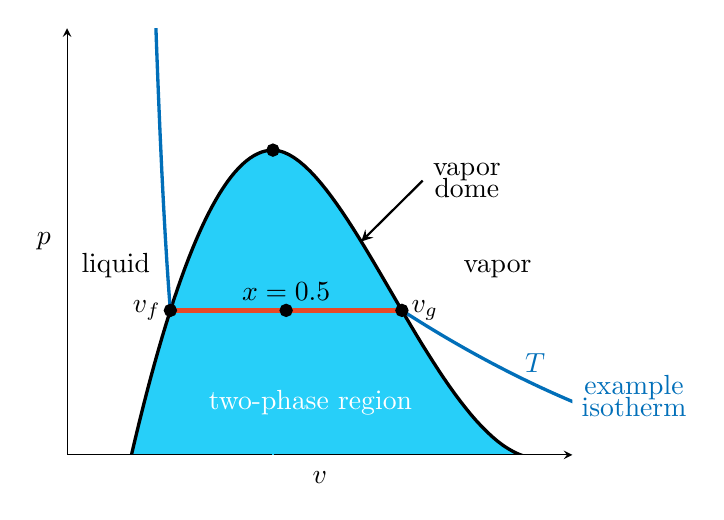
\begin{tikzpicture}[auto,every text node part/.style={align=center},
	declare function={
        		curveL(\x) = -0.7*\x^2+10;
		curveR(\x) = -1*\x^2 + 0.3*x^2.5 + 10;
		TcurveL(\x) = 2*(\x+1.5)^4;
		TcurveR(\x) = -1*x+7.83+0.03*x^2;
  	}
	]
	
% left plot
	\node (ref) at (0,0) [draw=none, coordinate] {};
	\begin{axis} [at={(ref)},xmin=-5.5, ymin=0, xmax=8, ymax = 14, samples = 50, 
			ytick=\empty, yticklabels={}, ylabel style={rotate=-90},
			xtick=\empty, xticklabels={},
			ylabel={$p$}, xlabel={$v$},
			width = 8cm, height=7cm, axis y line = left, axis x line = bottom,
			thick, fill between/on layer={axis background}]
		%L+V dome
		\addplot[very thick,domain=-5:0, name path=L] {curveL(x)};	
		\path[name path=axL] (axis cs:-5, 0) -- (axis cs:0, 0);	
		\addplot[very thick,domain=0:7, name path=R] {curveR(x)};
		\path[name path=axR] (axis cs:0, 0) -- (axis cs:14, 0);
		\addplot [fill=Dteal]
		fill between [
			of = L and axL,
			soft clip={domain=-5:0},
		];
		\addplot [fill=Dteal]
		fill between [
			of = R and axR,
			soft clip={domain=0:14},
		];
		\addplot[color=Dteal] coordinates {(0,10) (0,0)}; % cover seam
		
		% points
		\addplot[mark=*] coordinates {(0,10)};
		\addplot[mark=*] coordinates {(-2.74,4.74142)} node[left]{$v_f$};
		\addplot[mark=*] coordinates {(3.4445,4.74142)} node[right]{$v_g$};
		\addplot[mark=*] coordinates {(0.352,4.74142)} node[above]{$x = 0.5$};
		
		% isotherm 
		\addplot[very thick,domain=-5:-2.74, Dlblue] {TcurveL(x)};	
		\addplot[ultra thick,domain=-2.74:3.4445,Dorange] {4.74142};
		\addplot[very thick,domain=3.44449:14, Dlblue] {TcurveR(x)};	
		
		% vf vg labels

		

		\node [above, color=black] at (axis cs:6, 5.5) {vapor};
		\node [above, color=black] at (axis cs:-4.2, 5.5) {liquid};
		\node [color=Dlblue] at (axis cs:7, 3) {$T$};
		\node [above,color=white] at (axis cs:1, 1) {two-phase region};
		\draw [thick,stealth-] (axis cs:2.35863, 7) -- (axis cs:4, 9) node[right]{vapor\\[-4pt]  dome};
		%\node [above, color=black] at (axis cs:0.5, 0.2) {$\int_{V_1}^{V_2} p dV = $\hspace{6pt} \\ \hspace{18pt}$p (V_2-V_1)$};
		%\node [above, color=black] at (axis cs:0.5, 0.68) {process ${1\rightarrow2}$};

	\end{axis}
	\node (isolabel) at ($(ref)+(7.2,0.75)$) [draw=none,color=Dlblue]{example \\[-4pt]isotherm};

\end{tikzpicture}\end{center}
\caption{A $pv$ liquid-vapor phase diagram for a pure substance illustrating thermodynamic properties that define the two-phase region. }\label{fig:PhaseDiag2phase}
\end{figure}
\paragraph{Supercritical Fluid:} Phase of the substance when existing above the critical point, and possesses characteristics similar to both liquids and gases, but strictly behaves as neither.
\paragraph{Isotherm:} For a given $p$ and $v$, the substance's $T$ lies on an isotherm. The segment of the isotherm within the vapor dome is \textbf{horizontal} because phase transitions occur at a constant $T$ and $p$.

\paragraph{State of a Substance:} If any two independent intensive variables are known ($T, v, p, x, h, u$), they fix the \textbf{state} of the substance. (Intensive variables are independent of mass. For example, specific volume $v$ is intensive. Volume $V=mv$ is not.)


\subsubsection{Critical Values and Ideal Gases}
Ideal gases are modeled as having internal energy entirely composed of kinetic energy due to the absence of any interactions between the particles of the gas, which occurs when:
\begin{enumerate}
    \item The particles are far away from each other, at lower pressure or density 
    \item the kinetic energy of the particles is so large as to render the energy due to interactions between them negligible, at high temperature
\end{enumerate}
\paragraph{Reduced Values:}
\emph{Low} and \emph{high} are relative terms and depend on the particular gas, specifically its phase behavior.  Reduced values are normalized with respect to their values at the critical point to describe where gases are far enough away from the vapor dome to behave ideally,
($p_c$, $v_c$, and $T_c$). The following expressions 
\begin{equation}
p_R = p/p_c \qquad T_R = T/T_c \qquad v_R' = \frac{v}{R(T_c/p_c)}
\end{equation}
define the \textbf{reduced pressure}, \textbf{reduced temperature}, and \textbf{pseudoreduced specific volume}.
\paragraph{Compressibility factor:} The compressibility factor, $Z$, for an ideal gas equals 1, meaning a gas behaves ideally at infinitely small $p$. Therefore, the more deviation of Z from unity the less ideally a gas behaves.
\begin{equation}\label{eq:Z}
Z = \frac{pv}{RT}
\end{equation}


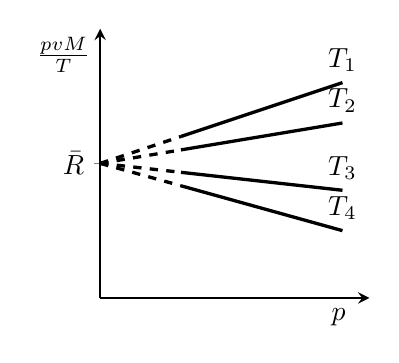
\begin{tikzpicture}[auto,every text node part/.style={align=center}]
% left plot
	\node (ref) at (0,0) [draw=none, coordinate] {};
	\begin{axis} [at={(ref)},xmin=0, ymin=-5, xmax=10, ymax = 5, samples = 50, 
			ytick=0, yticklabels={$\bar{R}$}, ylabel style={rotate=-90},
			xtick=\empty, xticklabels={},
			ylabel={$\frac{pvM}{T}$}, xlabel={$p$},
			width = 5cm, height=5cm, axis y line = left, axis x line = bottom,
			thick, fill between/on layer={axis background},ylabel style = {at={(axis description cs:0,0.8)},anchor=south east},
			xlabel style = {at={(axis description cs:0.95,0)},anchor=north east}]

		\addplot[very thick,dashed] coordinates {(0,0) (3,1)};
		\addplot[very thick] coordinates {(3,1) (9,3)} node[above]{$T_1$};
		\addplot[very thick,dashed] coordinates {(0,0) (3,0.5)};
		\addplot[very thick] coordinates {(3,0.5) (9,1.5)} node[above]{$T_2$};
		\addplot[very thick,dashed] coordinates {(0,0) (3,-0.333)};
		\addplot[very thick] coordinates {(3,-0.333) (9,-1)} node[above]{$T_3$};
		\addplot[very thick,dashed] coordinates {(0,0) (3,-0.833)};
		\addplot[very thick] coordinates {(3,-0.833) (9,-2.5)} node[above]{$T_4$};

	\end{axis}

\end{tikzpicture}
%%%%%%%%%%%%%%%%%%%%%%%%%%%%%%%%%%%%%%%%%%%%%%%%%%%%%%%%%%%%%%%%%%%%%%%%%%%%%%%%%%%%%%%%%%%%%%%%%%%%%%%%%%%%%%%%%%%%%%%%%%%%%%%%%%%%%%%
\subsection{Ideal Gases}
A gas is a state of matter that has neither independent shape nor volume. When contained, the atoms or molecules that comprise it interact with every boundary of the container.
\subsubsection{Ideal Gas Assumptions}
An ideal gas is a hypothetical model of a gas that follows the assumptions that
\begin{itemize}
	\item molecules are infinitesimally small (just points in space)
    \begin{itemize}
        \item ideal gas molecules never collide with one another
        \item ideal gas molecules occupy no volume
    \end{itemize} 
	\item intermolecular forces are zero
    \begin{itemize}
        \item ideal gas molecules  have no potential energies between molecules
        \item internal energy is only a function of kinetic energy
    \end{itemize}
\end{itemize}
\vspace{12pt}

\begin{figure}[h]
\begin{center}
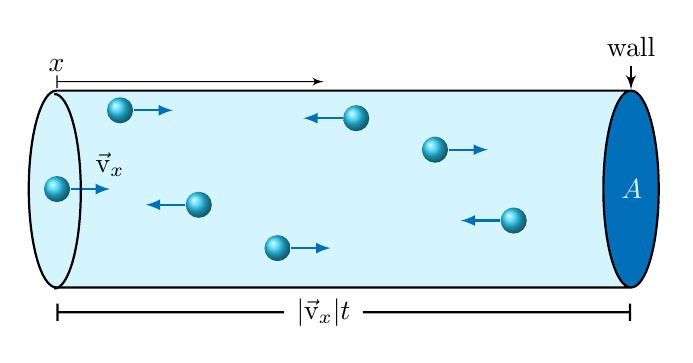
\begin{tikzpicture}[auto, >=latex']
	% Cylinder
  \node [cylinder,draw=black, thick,aspect=3,minimum height=8cm,minimum width=2.5cm,shape border rotate=0,cylinder uses custom fill, cylinder body     fill=Lteal,cylinder end fill=Dlblue] (A) {};
    % particle end
     \node [circle,draw=none, minimum width=5pt, ball color=Dteal, right=0.2cm of A.bottom] (p) {};
    \node[coordinate, right=0.5cm of p] (pend) {};
     	\draw [-latex, thick, draw=Dlblue] (p) -- (pend);
	    % particle end
     \node [circle,draw=none, minimum width=5pt, ball color=Dteal, right=1cm of A.bottom, yshift=1cm] (p2) {};
    \node[coordinate, right=0.5cm of p2] (pend2) {};
     	\draw [-latex, thick, draw=Dlblue] (p2) -- (pend2);
	    % particle end
     \node [circle,draw=none, minimum width=5pt, ball color=Dteal, right=3cm of A.bottom, yshift=-0.75cm] (p3) {};
    \node[coordinate, right=0.5cm of p3] (pend3) {};
     	\draw [-latex, thick, draw=Dlblue] (p3) -- (pend3);
	    % particle end
     \node [circle,draw=none, minimum width=5pt, ball color=Dteal, right=5cm of A.bottom, yshift=0.5cm] (p4) {};
    \node[coordinate, right=0.5cm of p4] (pend4) {};
     	\draw [-latex, thick, draw=Dlblue] (p4) -- (pend4);
	    % particle end
     \node [circle,draw=none, minimum width=5pt, ball color=Dteal, right=2cm of A.bottom, yshift=-0.2cm] (p5) {};
    \node[coordinate, left=0.5cm of p5] (pend5) {};
     	\draw [-latex, thick, draw=Dlblue] (p5) -- (pend5);
	    % particle end
     \node [circle,draw=none, minimum width=5pt, ball color=Dteal, right=4cm of A.bottom, yshift=0.9cm] (p6) {};
    \node[coordinate, left=0.5cm of p6] (pend6) {};
     	\draw [-latex, thick, draw=Dlblue] (p6) -- (pend6);
	    % particle end
     \node [circle,draw=none, minimum width=5pt, ball color=Dteal, right=6cm of A.bottom, yshift=-0.4cm] (p7) {};
    \node[coordinate, left=0.5cm of p7] (pend7) {};
     	\draw [-latex, thick, draw=Dlblue] (p7) -- (pend7);
     % other cylinder end
    \draw[solid, thick]
    let \p1 = ($ (A.after bottom) - (A.before bottom) $),
        \n1 = {0.5*veclen(\x1,\y1)-\pgflinewidth},
        \p2 = ($ (A.bottom) - (A.after bottom)!.5!(A.before bottom) $),
        \n2 = {veclen(\x2,\y2)-\pgflinewidth}
  in
    ([xshift=-\pgflinewidth] A.before bottom) arc [start angle=270, delta angle=180,
    x radius=\n2, y radius=\n1];	
    % Nodes for lines and labels
    \node[coordinate, above=0.1 cm of A.north] (xend) {};
    \node[coordinate, below=0.3 cm of A.before bottom] (D1) {};
    \node[coordinate, below=0.3 cm of A.after top] (D2) {};
    \node[coordinate, below=0.3 cm of A.south, xshift=-0.5cm] (D3) {};
    \node[coordinate, below=0.3 cm of A.south, xshift=0.5cm] (D4) {};
    \node[below=0 cm of A.south] {$|\vec{\textrm{v}}_x|t$};
    % Labels
	\node(area1) [draw=none, fill=none, left=0.1cm of A.top]{\textcolor{Lteal}{$A$}};
	\node(wall) [draw=none, fill=none, above=0.3cm of A.before top]{wall};
	\node(x)  [draw=none, fill=none, above=0.1cm of A.after bottom]{$x$};
	\node [draw=none, fill=none, above=1pt of pend] {$\vec{\textrm{v}}_x$};
	%\node(1) [draw=none, fill=none, right=0.1cm of B.east, yshift=0.7cm]{$\mathcal{B}_B$};
	% Lines and arrows
	\draw [->, thick] (wall) -- (A.before top);
	\draw [|->] (x.south) -- (xend);
	\draw [|-, thick] (D1) -- (D3);
	\draw [|-, thick] (D2) -- (D4);
\end{tikzpicture}
\end{center}
\caption{A sub-volume of gas next to a sub-section of the container wall having area, $A$.}\label{fig:IGequil}
\end{figure}

\subsubsection{Equation of State}
It has been shown empirically that an ideal gas obeys the \textbf{equation of state} 
\begin{equation}\label{eq:IGeos}
pV=n\overline{R}T
\end{equation}

\begin{equation*}
\overline{R} = \begin{cases} 
	&8.314 \textrm{ kJ/kmol}\cdot\textrm{K}\\
	&1.986 \textrm{ Btu/lbmol}\cdot\textrm{$^{\circ}$R}\\
	&1545 \textrm{ ft$\cdot$lbf/kmol}\cdot\textrm{$^{\circ}$R}\\
	\end{cases}
\end{equation*}
\subsubsection{Temperature Effects}
$\overline{R}$ defines the proportionality constant that converts the average translational kinetic energy of a single particle, $\langle KE\rangle $, to temperature ($N_A$ is Avagadro's number)
\begin{equation}
T = \frac{2}{3} \frac{N_A}{\overline{R}}\langle KE \rangle.
\end{equation}


Internal energy \underline{of an ideal gas} depends only on the total molecular kinetic energy.  Therefore, internal energy is solely a function of the temperature, $T$, and mass of the gas, $m$. The rate of change of the specific internal energy, $u$, where $u = U/m$, of an ideal gas with respect to $T$ is its constant volume specific heat, $c_v$
\begin{equation}
\frac{du}{dT} = c_v
\end{equation}
It follows that the change in internal energy of an ideal gas due to a change in temperature from $T_1$ to $T_2$ is given by
\begin{equation}
\Delta U = U_2 - U_1 = m\int_{T_1}^{T_2} c_v dT.
\end{equation}
%%%%%%%%%%%%%%%%%%%%%%%%%%%%%%%%%%%%%%%%%%%%%%%%%%%%%%%%%%%%%%%%%%%%%%%%%%%%%%%%%%%%%%%%%%%%%%%%%%%%%%%%%%%%%%%%%%%%%%%%%%%%%%%%%%%%
\subsection{\teal{Incompressible Fluids}}
In the \textbf{incompressible substance model}, the volume of a quantity of a substance cannot be compressed or expanded, thus its specific volume is constant. \subsubsection{Internal Energy of Incompressible Fluids}
Because the specific volume is not changing, the average intermolecular potential energy, which from the average distance between molecules, cannot change. Thus, the only contribution to an incompressible substance's internal energy comes from atomic and molecular kinetic energy, quantified via temperature. It follows that, like the ideal gas model, the \emph{internal energy of an incompressible substance is a function of temperature only} and 
    \begin{equation*}
        u = u(T)
    \end{equation*}
    \begin{equation*}
        \label{eqn:cvDefinition}
        \frac{du}{dT} = c_v.
    \end{equation*}
\subsubsection{Specific Heat of Incompressible Fluids}
For an incompressible substance, \emph{constant pressure specific heat} $c_p$ equals \emph{constant volume specific heat} $c_v$. $c_p$ is defined as the partial derivative of the enthalpy $h$, while pressure $p$ is held constant.
    \begin{equation*}
        c_p \equiv \left(\frac{\partial h}{\partial T}\right)_p.
    \end{equation*}
By definition $h = u+pv$, thus at constant $p$ and for an incompressible substance (constant $v$), we can write the partial derivative of $h$ with respect to $T$ as
    \begin{equation*}
        \left(\frac{\partial h}{\partial T}\right)_p = \left(\frac{\partial u}{\partial T}\right)_p = \frac{du}{dT} = c_v
    \end{equation*}
where the conversion from a partial to total derivative arises because $u = u(T)$ for an incompressible substance. Therefore $c_p = \left(\frac{\partial h}{\partial T}\right)_p = c_v$ for an incompressible substance.
    \begin{equation*}
        c_p = c_v = c
    \end{equation*}
\subsubsection{Specific Entropy Change of Incompressible Fluids}
For an \emph{ideal gas} with a given, \textbf{constant specific heat $c_v$}, its change in specific entropy from a state $1$ to a state $2$ is given by the expression
    \begin{equation*}
        s_2 - s_1 = c_v\ln\frac{T_2}{T_1}+ R \ln\frac{v_2}{v_1}
    \end{equation*}
where $R$ is the gas constant and $v$ is the specific volume. Assuming this ideal gas is incompressible, $v_2=v_1$.  Therefore, 
    \begin{equation*}
        s_2 - s_1 = c_v\ln\frac{T_2}{T_1}+ R \ln(1)
    \end{equation*}
the ratio of $\frac{v_2}{v_1}=1$ and the $ln(1)=0$, simplifying the change in specific entropy is 
    \begin{equation*}
        s_2 - s_1 = c\ln\frac{T_2}{T_1},
    \end{equation*}
as long as $c$ is constant.
    



\section{Energy Transfers}\label{sec:energytransfers}
When mass does not flow into or out of a system, the energy of the system changes in only two ways, through the loss or addition of \textbf{work} and/or \textbf{heat}.

\noindent The internal energy ($U$) of a system is affected by the energetic contributions from heat flow ($Q$) in and out of a system and work ($W$)done by or on a system.  
\begin{equation}\label{eq:Ebal}
\Delta U = Q -  W.
\end{equation}
\begin{figure}[h]
\begin{center}
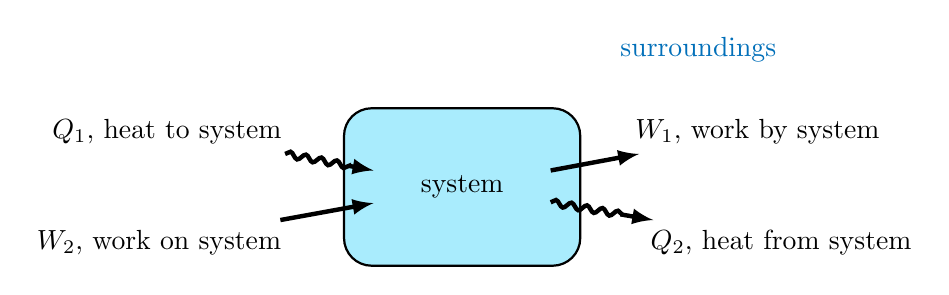
\begin{tikzpicture}[auto, node distance=1.75cm,>=latex']
	\node(1) [draw, fill=Mteal, rectangle, rounded corners=10pt, minimum width=3cm, minimum height = 2cm, text centered,thick] {system};
	\node(100) [draw=none, fill=none, text width=2cm, text height=0.5cm, text depth=0.5cm]{};
	% Flow labels
	\node(2) [draw=none, fill=none, left of=1,yshift=0.7cm, xshift=-2cm]{$Q_{1}$, heat to system};
	\node(3) [draw=none, fill=none, left of=1,yshift=-0.7cm, xshift=-2.1cm]{$W_{2}$, work on system};
	\node(4) [draw=none, fill=none, right of=1,yshift=-0.7cm, xshift=2.3cm]{$Q_{2}$, heat from system};
	\node(5) [draw=none, fill=none, right of=1,yshift=0.7cm, xshift=2cm]{$W_{1}$, work by system};
	\node(6) [draw=none, fill=none, above of=1,xshift = 3cm]{\color{Dlblue}surroundings};
	% Flow arrows
	\draw [-latex,decorate,decoration={snake,amplitude=.4mm,segment length=2mm, post length=9pt}, ultra thick] (2) -- (100);
	\draw[-latex,decorate,decoration={snake,amplitude=.4mm,segment length=2mm ,post length=9pt}, ultra thick] (100) -- (4);
	\draw [-latex, ultra thick] (3) -- (100);
	\draw [-latex, ultra thick] (100) -- (5);
\end{tikzpicture}
\end{center}
\caption{A schematic illustrating the direction of energy flow when heat is transferred to/from the system and work is performed on or by the system.}\label{fig:SysSchematic1}	
\end{figure}
%%%%%%%%%%%%%%%%%%%%%%%%%%%%%%%%%%%%%%%%%%%%%%%%%%%%%%%%%%%%%%%%%%%%%%%%%%%%%%%%%%

\subsection{Heat}
In thermodynamics, heat $Q$ is the thermal energy transferred between systems due to a temperature difference. Heat can both flow into and out of a system as shown in Figure \ref{fig:HeatSchematic}.


\begin{figure}[h]
\begin{center}
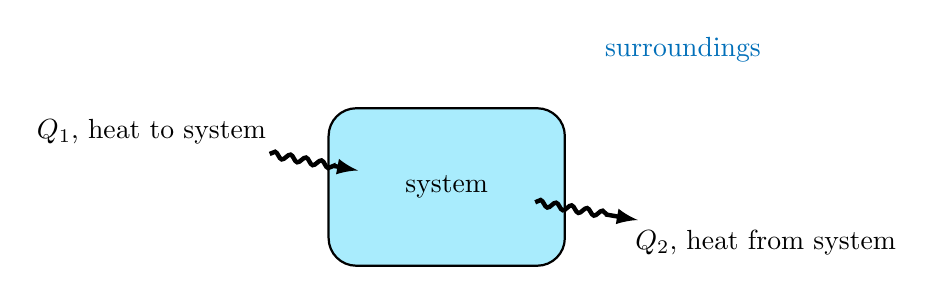
\begin{tikzpicture}[auto, node distance=1.75cm,>=latex']
	\node(1) [draw, fill=Mteal, rectangle, rounded corners=10pt, minimum width=3cm, minimum height = 2cm, text centered,thick] {system};
	\node(100) [draw=none, fill=none, text width=2cm, text height=0.5cm, text depth=0.5cm]{};
	% Flow labels
	\node(2) [draw=none, fill=none, left of=1,yshift=0.7cm, xshift=-2cm]{$Q_{1}$, heat to system};
	\node(3) [draw=none, fill=none, right of=1,yshift=-0.7cm, xshift=2.3cm]{$Q_{2}$, heat from system};
	\node(4) [draw=none, fill=none, above of=1,xshift = 3cm]{\color{Dlblue}surroundings};
	% Flow arrows
	\draw [-latex,decorate,decoration={snake,amplitude=.4mm,segment length=2mm, post length=9pt}, ultra thick] (2) -- (100);
	\draw[-latex,decorate,decoration={snake,amplitude=.4mm,segment length=2mm ,post length=9pt}, ultra thick] (100) -- (3);
\end{tikzpicture}
\end{center}
\caption{A schematic illustrating the heat flow transferred to/from the system.}\label{fig:HeatSchematic}	
\end{figure}
%%%%%%%%%%%%%%%%%%%%%%%%%%%%%%%%%%%%%%%%%%%%%%%%%%%%%%%%%%%%%%%%%%%%%%%%%%%%%%%%%%

%%%%%%%%%%%%%%%%%%%%%%%%%%%%%%%%%%%%%%%%%%%%%%%%%%%%%%%%%
%%%%%%%%%%%%%%%%%%%%%%%%%%%%%%%%%%%%%%%%%%%%%%%%%%%%%%%%%
\subsection{Work}
Recall from previous physics courses, that when a force $f$ acts over a distance $d$ it does work, defined as
\begin{equation}
W=fd.
\end{equation}
However, applied force does not have to be constant during a process. More generally, work is
\begin{equation}
\label{eqn: GenW}
W=\int_{d_1}^{d_2}f(x)dx
\end{equation}
where $f$ varies along the path parameterized by $x$ from position $d_1$ to position $d_2$, where we are assuming $f$ is tangent to the path.
 

%%%%%%%%%%%%%%%%%%%%%%%%%%%%%%%%%%%%%%%%%%%%%%%%%%%%%%%%%%%%%%%%%%%%%%%%%%%%%%%%%%%%%%%%

\subsubsection{$pV$ work}
Work done by or on a gas, is known as $\boldsymbol{pV}$~\textbf{work}.  A gas, such as the one enclosed in the cylindrical device in Figure \ref{fig:pressure}, applies a force uniformly over an area $A$, due to collisions against the wall, which is defined as pressure,
\begin{figure}[h]
\begin{center}
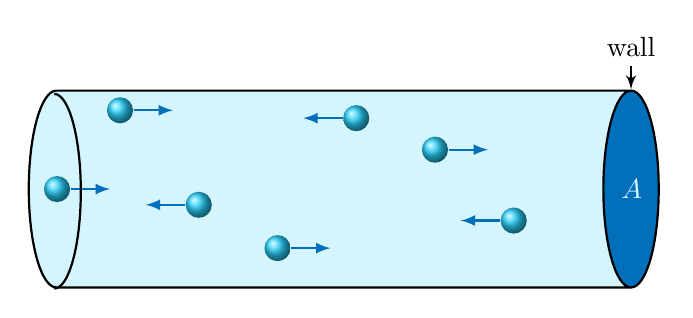
\begin{tikzpicture}[auto, >=latex']
	% Cylinder
  \node [cylinder,draw=black, thick,aspect=3,minimum height=8cm,minimum width=2.5cm,shape border rotate=0,cylinder uses custom fill, cylinder body     fill=Lteal,cylinder end fill=Dlblue] (A) {};
    % particle end
     \node [circle,draw=none, minimum width=5pt, ball color=Dteal, right=0.2cm of A.bottom] (p) {};
    \node[coordinate, right=0.5cm of p] (pend) {};
     	\draw [-latex, thick, draw=Dlblue] (p) -- (pend);
	    % particle end
     \node [circle,draw=none, minimum width=5pt, ball color=Dteal, right=1cm of A.bottom, yshift=1cm] (p2) {};
    \node[coordinate, right=0.5cm of p2] (pend2) {};
     	\draw [-latex, thick, draw=Dlblue] (p2) -- (pend2);
	    % particle end
     \node [circle,draw=none, minimum width=5pt, ball color=Dteal, right=3cm of A.bottom, yshift=-0.75cm] (p3) {};
    \node[coordinate, right=0.5cm of p3] (pend3) {};
     	\draw [-latex, thick, draw=Dlblue] (p3) -- (pend3);
	    % particle end
     \node [circle,draw=none, minimum width=5pt, ball color=Dteal, right=5cm of A.bottom, yshift=0.5cm] (p4) {};
    \node[coordinate, right=0.5cm of p4] (pend4) {};
     	\draw [-latex, thick, draw=Dlblue] (p4) -- (pend4);
	    % particle end
     \node [circle,draw=none, minimum width=5pt, ball color=Dteal, right=2cm of A.bottom, yshift=-0.2cm] (p5) {};
    \node[coordinate, left=0.5cm of p5] (pend5) {};
     	\draw [-latex, thick, draw=Dlblue] (p5) -- (pend5);
	    % particle end
     \node [circle,draw=none, minimum width=5pt, ball color=Dteal, right=4cm of A.bottom, yshift=0.9cm] (p6) {};
    \node[coordinate, left=0.5cm of p6] (pend6) {};
     	\draw [-latex, thick, draw=Dlblue] (p6) -- (pend6);
	    % particle end
     \node [circle,draw=none, minimum width=5pt, ball color=Dteal, right=6cm of A.bottom, yshift=-0.4cm] (p7) {};
    \node[coordinate, left=0.5cm of p7] (pend7) {};
     	\draw [-latex, thick, draw=Dlblue] (p7) -- (pend7);
     % other cylinder end
    \draw[solid, thick]
    let \p1 = ($ (A.after bottom) - (A.before bottom) $),
        \n1 = {0.5*veclen(\x1,\y1)-\pgflinewidth},
        \p2 = ($ (A.bottom) - (A.after bottom)!.5!(A.before bottom) $),
        \n2 = {veclen(\x2,\y2)-\pgflinewidth}
  in
    ([xshift=-\pgflinewidth] A.before bottom) arc [start angle=270, delta angle=180,
    x radius=\n2, y radius=\n1];	
    % Nodes for lines and labels
    \node[coordinate, above=0.1 cm of A.north] (xend) {};
    \node[coordinate, below=0.3 cm of A.before bottom] (D1) {};
    \node[coordinate, below=0.3 cm of A.after top] (D2) {};
    \node[coordinate, below=0.3 cm of A.south, xshift=-0.5cm] (D3) {};
    \node[coordinate, below=0.3 cm of A.south, xshift=0.5cm] (D4) {};
    
    % Labels
	\node(area1) [draw=none, fill=none, left=0.1cm of A.top]{\textcolor{Lteal}{$A$}};
	\node(wall) [draw=none, fill=none, above=0.3cm of A.before top]{wall};
	%\node(1) [draw=none, fill=none, right=0.1cm of B.east, yshift=0.7cm]{$\mathcal{B}_B$};
	% Lines and arrows
	\draw [->, thick] (wall) -- (A.before top);
	
	
\end{tikzpicture}
\end{center}
\caption{A sub-volume of gas, imparting forces from collisions on a sub-section of the container wall having area, $A$.}\label{fig:pressure}
\end{figure}
\begin{equation}\label{eq:Pdefn}
p=\frac{f}{A}.
\end{equation}
Referring back to the definition of work in Eqn.~\ref{eqn: GenW}, if $x$ is a single cartesian direction normal to an area $A$ then $A\cdot dx$ is a differential volume $dV$.  Additionally, using the definition of pressure Eqn.~\ref{eq:Pdefn}, we can define $pV$ work as follows,
\begin{align}
\label{eq:pVwork}
W&=\int_{d_1}^{d_2}f(x)\,dx \nonumber \\
&=\int_{d_1}^{d_2}\frac{f(x)}{A}A\,dx \nonumber \\
&=\int_{V_1}^{V_2}p(V)\,dV 
\end{align}


\paragraph{$pV$ diagrams} Graphs whose $y$ and $x$ axes are $p$ and $V$, respectively.  According to Eqn.~\eqref{eq:pVwork}, work is the area under the process curve.  An example is shown in Figure \ref{fig:PVdiagrams}.

\begin{figure}[h]
\begin{center}
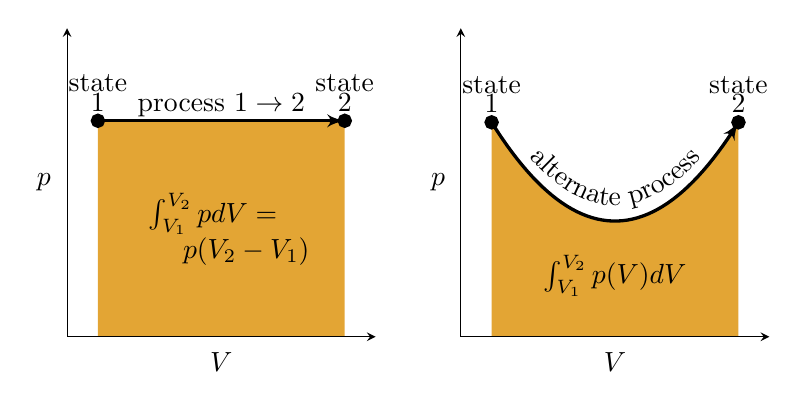
\begin{tikzpicture}[auto,>=latex',every text node part/.style={align=center},
	declare function={
        		curve(\x) = \x^2+0.75;
  	}
	]
	
% left plot
	\node (ref) at (0,0) [draw=none, coordinate] {};
	\begin{axis} [at={(ref)},xmin=0, ymin=0, xmax=1, ymax = 1, samples = 2, 
			ytick=\empty, yticklabels={}, ylabel style={rotate=-90},
			xtick=\empty, xticklabels={},
			ylabel={$p$}, xlabel={$V$},
			width = 5.5cm, height=5.5cm, axis y line = left, axis x line = bottom,
			domain = 0.1:0.9, thick, fill between/on layer={axis background}]
		
		\addplot[-> ,mark=*, very thick, name path=f] {0.7};		
		\path[name path=ax] (axis cs:0, 0) -- (axis cs:1, 0);
		\addplot [fill=Dlorange]
		fill between [
			of = f and ax,
			soft clip={domain=0.1:0.9},
		];
		\node [above, color=black] at (axis cs:0.1, 0.7) {state \\[-5pt]$1$};
		\node [above, color=black] at (axis cs:0.9, 0.7) {state \\[-5pt]$2$};
		\node [above, color=black] at (axis cs:0.5, 0.2) {$\int_{V_1}^{V_2} p dV = $\hspace{6pt} \\ \hspace{18pt}$p (V_2-V_1)$};
		\node [above, color=black] at (axis cs:0.5, 0.68) {process ${1\rightarrow2}$};


		
	\end{axis}

% right plot
	\node (ref2) at ($ (ref) + (5,0)$) [draw=none, coordinate] {};
	\begin{axis} [at={(ref2)},xmin=-1, ymin=0, xmax=1, ymax = 2, samples = 50, 
			ytick=\empty, yticklabels={}, ylabel style={rotate=-90},
			xtick=\empty, xticklabels={},
			ylabel={$p$}, xlabel={$V$},
			width = 5.5cm, height=5.5cm, axis y line = left, axis x line = bottom,
			domain = -0.8:0.8, fill between/on layer={axis background}]
		
		\addplot[name path=g, black, very thick,->] {curve(x)};
		\addplot[draw=none,decoration={text along path, text align=center, text={alternate process},}, postaction={decorate}]  {curve(x)+0.1};%mark options={decoration={name=none}} <- not needed here, but might be sometimes.
		\path[name path=ax2] (axis cs:-1, 0) -- (axis cs:1, 0);
		\addplot [fill=Dlorange]
		fill between [
			of = g and ax2,
			soft clip={domain=-0.8:0.8},
		];
		\addplot [only marks, very thick] coordinates {
		(-0.8, {curve(-0.8)})
		(0.8, {curve(0.8)})
		};
		\node [above, color=black] at (axis cs:-0.8, {curve(-0.8)}) {state \\[-5pt]$1$};
		\node [above, color=black] at (axis cs:0.8, {curve(0.8)}) {state \\[-5pt]$2$};
		\node [above, color=black] at (axis cs:0, 0.2) {$\int_{V_1}^{V_2} p(V) dV$};
		
	\end{axis}

\end{tikzpicture}
\end{center}
\caption{$pV$ diagrams for 2 processes where the start and end state are identical but with differing processes.}\label{fig:PVdiagrams}
\end{figure}

\paragraph{Isobaric Process:} During the process to go from 1 state to another, the system remains at a constant pressure, as shown in Figure \ref{fig:PVdiagrams} (left).

\paragraph{Work is path dependent:} Work transfer depends on the process. Figure \ref{fig:PVdiagrams} shows two processes where despite having the same initial and final thermodynamic states, the difference in magnitude of work for these two processes is different.


%%%%%%%%%%%%%%%%%%%%%%%%%%%%%%%%%%%%%%%%%%%%
%%%%%%%%%%%%%%%%%%%%%%%%%%%%%%%%%%%%%%%%%%%%
\subsubsection{\teal{Shaft work}}
\begin{figure}
\begin{center}
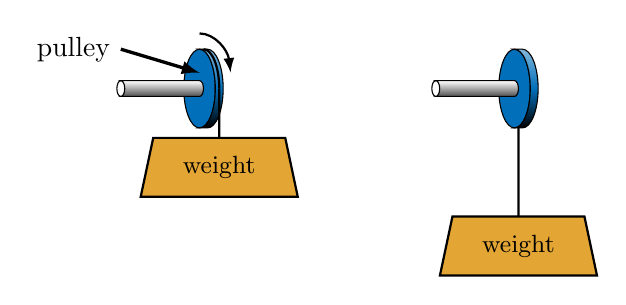
\begin{tikzpicture}[auto,every text node part/.style={align=center}]


	\draw[fill=Dlblue](0,0) circle (-0.2 and 0.5);
	\draw[top color=Dlblue!50,bottom color=black,middle color=Dlblue] (0.1,0.5) arc (90:270:-0.2 and 0.5) -- ++(-0.1,0) arc (-90:-270:-0.2 and 0.5) -- cycle;
	\draw[top color=white,bottom color=black!70] (0,1mm) arc (90:-90:0.5mm and 1mm)--++(-1cm,0) arc (-90:90:0.5mm and 1mm)-- cycle;
	%\draw[top color=white,bottom color=black!70] (0,3mm) arc (90:270:1.5mm and 3mm)--++(3cm,0) arc (-90:-270:1.5mm and 3mm)-- cycle;
	\draw (-1cm,1mm) arc (90:270:0.5mm and 1mm);

	\node (weight) at (0.25,-1) [draw, fill =Dlorange, trapezium, minimum width=2cm, trapezium angle =78,  outer sep=0pt, thick] {\small{weight}};
	\draw[thick] (0.05,0.5) arc (90:180:-0.2 and 0.5);
	\draw[thick] (0.25,0) -- (weight.north);
	
	\draw[thick, -latex] (0,0.7) arc (90:170:-0.4 and 0.6);
	
	\draw[very thick, -latex] (-1cm,0.5cm) node[left]{pulley}-- (0,0.2cm);
	

	\draw[fill=Dlblue](4,0) circle (-0.2 and 0.5);
	\draw[top color=Dlblue!50,bottom color=black,middle color=Dlblue] (4.1,0.5) arc (90:270:-0.2 and 0.5) -- ++(-0.1,0) arc (-90:-270:-0.2 and 0.5) -- cycle;
	\draw[top color=white,bottom color=black!70] (4,1mm) arc (90:-90:0.5mm and 1mm)--++(-1cm,0) arc (-90:90:0.5mm and 1mm)-- cycle;
	%\draw[top color=white,bottom color=black!70] (0,3mm) arc (90:270:1.5mm and 3mm)--++(3cm,0) arc (-90:-270:1.5mm and 3mm)-- cycle;
	\draw (3cm,1mm) arc (90:270:0.5mm and 1mm);

	\node (weight) at (4.05,-2) [draw, fill =Dlorange, trapezium, minimum width=2cm, trapezium angle =78,  outer sep=0pt, thick] {\small{weight}};
	\draw[thick] (4.05,-0.5) -- (weight.north);

\end{tikzpicture}\end{center}
\caption{Spontaneous lowering of a weight on a pulley.}\label{fig:WeightLower}
\end{figure}
Work can also be done via shaft work.  This can be explained by a shaft, on which a weight and pulley are mounted, providing a mechanism for inputting or extracting work as in Fig.~\ref{fig:CycleWithThermalReservoir}. Work $W_{\text{cycle}}$ is done by the lowering mass on the system when the mass is released from its the raised position. The motion of the molecules in the system increases due to the shaft work input. This additional molecular energy temporarily increases the temperature of the system before the excess thermal energy is transmitted as heat $Q$ to the reservoir.  
\begin{figure}
\begin{center}
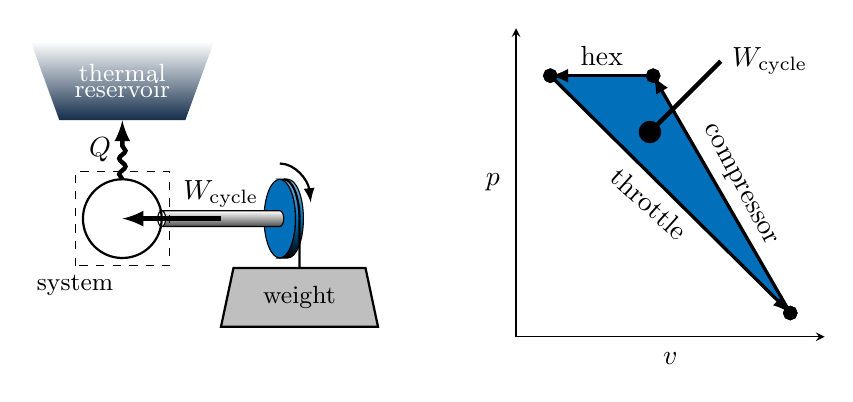
\begin{tikzpicture}[auto,every text node part/.style={align=center}]


	\draw[fill=Dlblue](0,0) circle (-0.2 and 0.5);
	\draw[top color=Dlblue!50,bottom color=black,middle color=Dlblue] (0.1,0.5) arc (90:270:-0.2 and 0.5) -- ++(-0.1,0) arc (-90:-270:-0.2 and 0.5) -- cycle;
	\draw[top color=white,bottom color=black!70] (0,1mm) arc (90:-90:0.5mm and 1mm)--++(-1.5cm,0) arc (-90:90:0.5mm and 1mm)-- cycle;
	%\draw[top color=white,bottom color=black!70] (0,3mm) arc (90:270:1.5mm and 3mm)--++(3cm,0) arc (-90:-270:1.5mm and 3mm)-- cycle;
	\draw (-1.5cm,1mm) arc (90:270:0.5mm and 1mm);

	\node (weight) at (0.25,-1) [draw, fill =gray!50, trapezium, minimum width=2cm, trapezium angle =78,  outer sep=0pt, thick] {\small{weight}};
	\draw[thick] (0.05,0.5) arc (90:180:-0.2 and 0.5);
	\draw[thick] (0.25,0) -- (weight.north);
	
	\draw[thick, -latex] (0,0.7) arc (90:170:-0.4 and 0.6);

	% system
	\draw[thick](-2,0) circle (0.5);
	\draw (-2.6,-0.6) node[below]{\small{system}} [thin,dashed] rectangle (-1.4,0.6);
	
	% thermal reservoir
	\node (Tres) at (-2,1.75) [draw=none, bottom color=Ddblue, top color=white, trapezium, minimum width=0cm, minimum height=1cm, outer sep=0pt,trapezium angle =70,  inner sep=5pt, inner xsep=8pt,thick,rotate=180] {};
	\node (Tlabel) at (Tres) [draw=none, text=white] {\small{thermal} \\[-6pt] \small{reservoir}};
	
	
	% heat & work flows
	\draw [ultra thick, -latex,decorate,decoration={snake,amplitude=.4mm,segment length=2mm, post length=9pt}] (-2,0.5) -- (Tres.north) node[midway]{$Q$} ;
	\draw [ultra thick, latex-] (-2,0) -- (-0.75,0) node[above]{$W_{\text{cycle}}$} ;
	
	
	\node (ref) at (3,-1.5) [draw=none, coordinate] {};
	\begin{axis} [at={(ref)},xmin=0.1, ymin=0.15, xmax=1, ymax = 0.8, samples = 2, 
			ytick=\empty, yticklabels={}, ylabel style={rotate=-90},
			xtick=\empty, xticklabels={},
			ylabel={$p$}, xlabel={$v$},
			width = 5.5cm, height=5.5cm, axis y line = left, axis x line = bottom,
			domain = 0.1:0.9, thick, fill between/on layer={axis background}]
		
		\addplot[-latex ,mark=*, very thick, name path=comp,domain=0.9:0.5] {0.2 -1.25*(x-0.9)};		
		\addplot[latex- ,mark=*, very thick, name path=throttle,domain=0.9:0.2] {0.2 -0.7143*(x-0.9)};	
		\addplot[-latex ,mark=*, very thick, name path=hex,domain=0.5:0.2] {0.7};	
		\addplot [fill=Dlblue]
		fill between [
			of = comp and throttle,
			soft clip={domain=0.1:0.9},
		];
		\node [above, color=black, rotate=-62] at (axis cs:0.7, 0.45) {compressor};
		\node [above, color=black, rotate=-42] at (axis cs:0.45, 0.4) {throttle};
		\node [above, color=black] at (axis cs:0.35, 0.7) {hex};
		
	\end{axis}

	\draw[ultra thick, *-] (4.6,1) -- (5.6,2) node[right]{$W_{\text{cycle}}$};

\end{tikzpicture}\end{center}
\caption{A cycle in contact with a single thermal reservoir (left) may operate such that work input leads to an equal amount of heat output. The $pv$ diagram for one such cycle (right) is shown for a compressor, heat exhanger (hex), and throttle running at steady state.}\label{fig:CycleWithThermalReservoir}
\end{figure}
\section{Mass and Energy Balances}
The rate of change of a system's internal energy is due to the net rate of energy input minus the net rate of energy output. 

\subsection{Closed System Energy Rate Balance} 
In the absence of mass flow, the closed system energy rate balance depends on the net heat flow rate $\dot{Q}(t)$ and the net work transfer rate $\dot{W}(t)$, as follows,
\begin{equation}\label{eqn:deltaIE}
\frac{dU}{dt}=\dot{Q}(t)-\dot{W}(t),
\end{equation}
%%%%%%%%%%%%%%%%%%%%%%%%%%%%%%%%%%%%%%%%%%%%%%%%%%%%%%%%%%%%%%%%%%%%%%%%%%%%%%%%%%%%%%%%%%%%%%%%%%%%%%%%%%%%%%%%%%%%%%%%%%%%%%%%%%%%%%
\begin{figure}[h]
\begin{center}
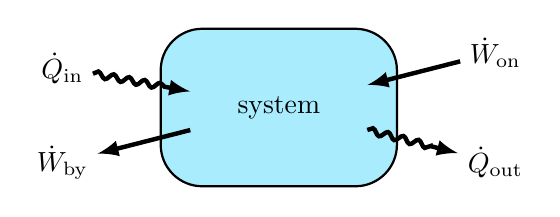
\begin{tikzpicture}[auto, node distance=1.75cm,>=latex']
	\node(1) [draw, fill=Mteal, rectangle, rounded corners=15pt, minimum width=3cm, minimum height = 2cm, text centered,thick] {system};
	\node(100) [draw=none, fill=none, text width=2cm, text height=0.5cm, text depth=0.5cm]{};
	% Flow labels
	\node(2) [draw=none, fill=none, left of=1,yshift=0.5cm, xshift=-1cm]{$\dot{Q}_{\text{in}}$};
	\node(5) [draw=none, fill=none, left of=1,yshift=-0.7cm, xshift=-1cm]{$\dot{W}_{\text{by}}$};
	\node(3) [draw=none, fill=none, right of=1,yshift=0.7cm, xshift=1cm]{$\dot{W}_{\text{on}}$};
	\node(4) [draw=none, fill=none, right of=1,yshift=-0.7cm, xshift=1cm]{$\dot{Q}_{\text{out}}$};
	% Flow arrows
	\draw [-latex,decorate,decoration={snake,amplitude=.4mm,segment length=2mm, post length=9pt}, ultra thick] (2) -- (100);
	\draw[-latex,decorate,decoration={snake,amplitude=.4mm,segment length=2mm ,post length=9pt}, ultra thick] (100) -- (4);
	\draw [-latex, ultra thick] (3) -- (100);
	\draw [-latex, ultra thick] (100) -- (5);
\end{tikzpicture}
\end{center}
\end{figure}

\paragraph{Net Heat Flow Rate:} Comprised of the sum of the heat flow rates into the system minus the flow rates out of the system. 
\begin{equation}
\label{eqn:dQdt}
\dot{Q}(t)=\dot{Q}_{\text{in}}(t)-\dot{Q}_{\text{out}}(t).
\end{equation}
\paragraph{Net Work Transfer Rate:} Also known as net \textbf{power} transfer, where $\dot{W}_{\text{by}}$ is the net work done by the system and $\dot{W}_{\text{on}}$ is the net work done on the system.
\begin{equation}
\label{eqn:dWdt}
\dot{W}(t)=\dot{W}_{\text{by}}-\dot{W}_{\text{on}}.
\end{equation}

\paragraph{Closed System Energy Rate Balance:} Here, $\dot{Q}_{\text{in}}$, $\dot{Q}_{\text{out}}$, $\dot{W}_{\text{by}}$ and $\dot{W}_{\text{on}}$ are explicitly defined as the \emph{magnitude} of energy flow in the direction stated. The rate of change of the internal energy in the system is determined by combining Eqns.~\ref{eqn:deltaIE}, ~\ref{eqn:dQdt}, and ~\ref{eqn:dWdt}.

\begin{equation}
\begin{split}
\frac{dU}{dt}&=\dot{Q}_{\text{in}}-\dot{Q}_{\text{out}}-(\dot{W}_{\text{by}}-\dot{W}_{\text{on}})\\
&=\dot{Q}_{\text{in}}-\dot{Q}_{\text{out}}-\dot{W}_{\text{by}}+\dot{W}_{\text{on}}
\end{split}
\end{equation}


\subsection{Closed System Energy Balance}
The previous expression for the closed system energy balance can be determined by integrating the closed system energy rate balance (Eqn.~\ref{eqn:deltaIE}) with respect to time,
\begin{equation}
\begin{split}
\label{eqn:intUdt}
U(t)-U(0)&=\int_0^t \dot{Q}(\tau)d\tau-\int_0^t \dot{W}(\tau)d\tau\\
\Delta U(t)&=Q(t)-W(t).
\end{split}
\end{equation}

\subsection{Energy Transfer via Mass Flow}
Energy also transfers to or from a system during mass flow. For mass flow into a system, energy increases by the addition of both the internal energy of the additional mass \emph{and} the $pV$ work done by the mass on the system as it enters, and vice versa.
%%%%%%%%%%%%%%%%%%%%%%%%%%%%%%%%%%%%%%%%%%%%%%%%%%%%%%%%%%%%%%%%%%%%%%%%%%%%%%%%%%%%%%%%%%%%%%%%%%%%%%%%%%%%%%%%%%%%%%%%%%%%%%%%
\begin{figure}[h]
\begin{center}
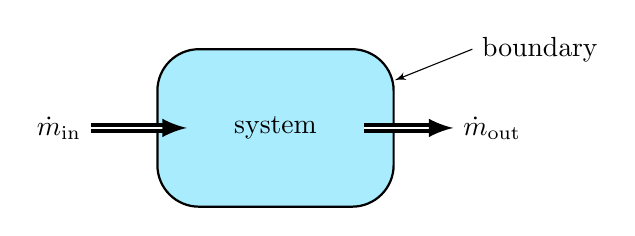
\begin{tikzpicture}[auto, node distance=1.75cm,>=latex']
	\node(1) [draw, fill=Mteal, rectangle, rounded corners=15pt, minimum width=3cm, minimum height = 2cm, text centered,thick] {system};
	\node(100) [draw=none, fill=none, text width=2cm, text height=0.5cm, text depth=0.5cm]{};
	% Flow labels
	\node(2) [draw=none, fill=none, left of=1,xshift=-1cm]{$\dot{m}_{\text{in}}$};
	\node(4) [draw=none, fill=none, right of=1,xshift=1cm]{$\dot{m}_{\text{out}}$};
	% Flow arrows
	\draw [-latex, double, ultra thick] (2) -- (100);
	\draw[-latex,double, ultra thick] (100) -- (4);t
	\draw[->] ($ (1) + (2.5,1)$) node[right]{boundary} -- (1);
\end{tikzpicture}
\end{center}
\end{figure}
%%%%%%%%%%%%%%%%%%%%%%%%%%%%%%%%%%%%%%%%%%%%%%%%%%%%%%%%%%%%%%%%%%%%%%%%%%%%%%%%%%%%%%%%%%%%%%%%%%%%%%%%%%%%%%%%%%%%%%%%%%%%%%%%
\begin{figure}
\begin{center}
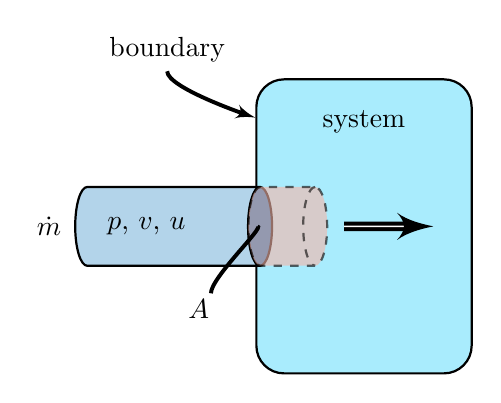
\begin{tikzpicture}[auto, node distance=1.75cm,>=latex']
	\node(1) [draw, fill=Mteal, rectangle, rounded corners=10pt, text width=2.5cm, text height = 0.5cm, text depth = 3cm, text centered,thick] {system};
	\node(100) [draw=none, fill=none, text width=2cm, text height=0.5cm, text depth=0.5cm]{};
	\node (2) [cylinder,thick,aspect=1.3,cylinder uses custom fill, cylinder body fill=Dlblue!30,cylinder end fill=Dlblue,shape border rotate=0, draw,minimum height=2.5cm,
	minimum width=1cm,xshift=-0.8cm,left of=1] { };
	\node(200) [draw=none, fill=none, right=0.3cm of 2.west]{$p$, $v$, $u$};
	\node (3) [cylinder,thick,aspect=1.3, fill=Dorange!40,opacity=0.6, dashed,shape border rotate=0, draw,minimum height=1cm,minimum width=1cm,left of=1,xshift=0.65cm]{};
	% Flow labels
	\node(201) [draw=none, fill=none, left of=2, xshift=0.3cm]{$\dot{m}$};
	\node(301) [draw=none, fill=none, below of=3, xshift=-1.0cm, yshift=0.7cm]{$A$};
	\node(101) [draw=none, fill=none, above of=1, xshift=-2.5cm, yshift=0.5cm]{boundary};
	% Flow arrows
	\draw [double,->, line width=0.5mm] ([xshift=0.2cm]3.east) -- ([xshift=-0.5cm]1.east);
	\draw [->, line width=0.5mm] (101) .. controls +(down:0.5cm) and +(left:0cm) .. ([yshift=-0.5cm]1.north west);
	\draw [-, line width=0.5mm] ([yshift=0.2cm,xshift=-0.1cm]301.east) .. controls +(up:0.2cm) and +(right:0.1cm) .. ([xshift=-0.2cm]2.east);
\end{tikzpicture}
\end{center}
\end{figure}
%%%%%%%%%%%%%%%%%%%%%%%%%%%%%%%%%%%%%%%%%%%%%%%%%%%%%%%%%%%%%%%%%%%%%%%%%%%%%%%%%%%%%%%%%%%%%%%%%%%%%%%%%%%%%%%%%%%%%%%%%%%%%%%%
\subsubsection{Internal Energy Change via Mass Flow}
A mass flow having rate $\dot{m}$ with cross-sectional area, $A$, \underline{slowly} enters a system. The mass is at a pressure $p$, has a specific volume $v$, and has a specific internal energy, $u$, relative to some reference state.
The mass flowing into the system, over a given time interval $\Delta t$, increases by the the internal energy the system as it enters, by:
\begin{equation}
\label{eqn:Deltau_dotm}
\dot{m}\Delta t u=mu.
\end{equation}

\subsubsection{$pV$ Work Done via Mass Flow}\label{sec:pvwork}
The volume occupied by the portion of the stream entering a system is defined by,
\begin{equation}
V_{\text{in-flow}}=\dot{m}\Delta t v=mv
\end{equation}
This volume is pushed at constant pressure, $p$, into the system, doing $pV$ work on the system,
\begin{equation}
\label{eqn:massflowPVwork}
W_{\text{in-flow}}=\int_{0}^{V_{\text{in-flow}}}p dV=mpv.
\end{equation}
For an input stream with a constant specific volume $v$ and pressure $p$, taking the derivative of the above expression with respect to time yields the rate of work  done on the system,
\begin{equation}
    \dot{W}=\dot{m}pv.
\end{equation}

\subsubsection{Total Internal Energy Change via Mass Flow}
It follows that the total increase in the internal energy of the system includes the contributions of both Eqn.~\ref{eqn:Deltau_dotm} and  Eqn.~\ref{eqn:massflowPVwork}.
\begin{equation}
\begin{split}
\Delta U&=mu+mpv\\
&=m(u+pv)
\end{split}
\end{equation}
The rate of internal energy increase is therefore,
\begin{equation}
\label{eqn:rateofDeltaU}
\frac{d U}{dt}=\dot{m}(u+pv)
\end{equation}
\subsubsection{Relative Specific Enthalpy}
Recall, that the sum $u+pv$ appears frequently in thermodynamic discussion so it is conveniently defined as relative specific enthalpy $h$, consisting of the same atomic and molecular kinetic and potential energies as specific internal energy $u$, but with the addition of \emph{flow work}, $pv$
\begin{equation}
\label{eqn:RelativeEnthalpy}
h=u+pv.
\end{equation}
%%%%%%%%%%%%%%%%%%%%%%%%%%%%%%%%%%%%%%%%%%%%%%%%%%%%%%%%%%%%%%%%%%%%%%%%%%%%%%%%%%%%%%%%%%%%%%%%%%%%%%%%%%%%%%%%%%%%%%%%%%%%%%%%

\subsection{Internal Energy Rate Balance}
In thermodynamic systems that experience both mass flow rates $\dot{m}_{\text{in}}$ and $\dot{m}_{\text{out}}$, net heat flow rate, $\dot{Q}$, into the system, and performs work at a rate $\dot{W}$ on its surroundings, a generalized energy rate balance can be used to describe all of these changes at once.
\begin{figure}[h]
\begin{center}
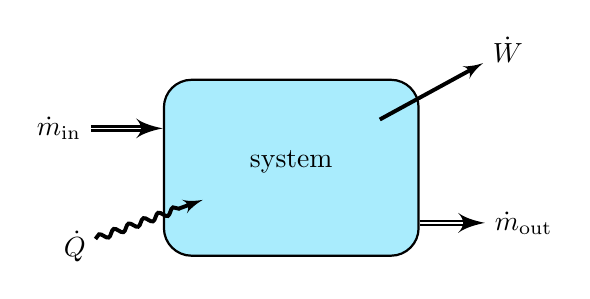
\begin{tikzpicture}[auto, node distance=1.75cm,>=latex']
	\node(1) [draw, fill=Mteal, rectangle, rounded corners=10pt, text width=3cm, text height = 1cm, text depth = 1cm, text centered,thick] {system};
	\node(100) [draw=none, fill=none, text width=2cm, text height=0.5cm, text depth=0.5cm]{};
	% Flow labels
	\node(2) [draw=none, fill=none, left of=1,yshift=0.5cm, xshift=-1.2cm]{$\dot{m}_{\text{in}}$};
	\node(3) [draw=none, fill=none, left of=1,yshift=-1cm, xshift=-1cm]{$\dot{Q}$};
	\node(4) [draw=none, fill=none, right of=1,yshift=1.5cm, xshift=1cm]{$\dot{W}$};
	\node(5) [draw=none, fill=none, right of=1,yshift=-0.7cm, xshift=1.2cm]{$\dot{m}_{\text{out}}$};
	% Flow arrows
	\draw [double,->, line width=0.3mm] (2) -- (2-|1.west);
	\draw[->, line width=0.5mm] (100) -- (4);
	\draw [->,decorate,decoration={snake,amplitude=.4mm,segment length=2mm ,post length=9pt}, line width=0.5mm] (3) -- (100);
	\draw [double,->, line width=0.3mm] (5-|1.east) -- (5);
\end{tikzpicture}
\end{center}
\caption{A schematic of an open system for which a net heat transfer rate $\dot{Q}$, a net power output $\dot{W}$, and mass flowrates into $\dot{m}_{\text{in}}$ and out of $\dot{m}_{\text{out}}$ the system occur.} \label{fig:OpenSystemQW}
\end{figure}
\vspace{12pt}

\textbf{Recall} that the rate of change of the internal energy of a system in the absence of mass flows is given by
\begin{equation}
\label{eqn:ROCofU_woMF}
\left.\frac{dU}{dt}\right|_{\text{no-flow}}=\dot{Q}(t)-\dot{W}(t)
\end{equation}
\vspace{12 pt}

\textbf{Recall} that the the mass flow rate `in' changes the internal energy of the system at a rate
\begin{equation}
\label{eqn:ROCofU_MFin}
\left.\frac{dU}{dt}\right|_{\text{in-flow}}=\dot{m}_{\text{in}}(u_{\text{in}}+p_{\text{in}}v_{\text{in}})=\dot{m}_{\text{in}}h_{\text{in}}
\end{equation}
\vspace{12 pt}

\textbf{Similarly} the mass flow rate `out' changes the internal energy at a rate
\begin{equation}
\label{eqn:ROCofU_MFout}
\left.\frac{dU}{dt}\right|_{\text{out-flow}}=-\dot{m}_{\text{out}}(u_{\text{out}}+p_{\text{out}}v_{\text{out}})=-\dot{m}_{\text{out}}h_{\text{out}}
\end{equation}
The total rate of change in the internal energy is the sum of Eqns.~\ref{eqn:ROCofU_woMF}, \ref{eqn:ROCofU_MFin}, and \ref{eqn:ROCofU_MFout}, yielding a generalized equation
to an arbitrary number of input and output streams yields
\begin{equation}
  \frac{dU}{dt}=\dot{Q}-\dot{W}+\sum_{\text{in}}\dot{m}_{\text{in}}h_{\text{in}}-\sum_{\text{out}}\dot{m}_{\text{out}}h_{\text{out}}  
\end{equation}
%%%%%%%%%%%%%%%%%%%%%%%%%%%%%%%%%%%%%%%%%%%%%%%%%%%%%%%%%%%%%%%%%%%%%%%%%%%%%%%%%%%%%%%%%%%%%%%%%%%%%%%%%%%%%%%%%%%%%%%%%%%%%%%%
\subsection{Total Energy Balance}
The kinetic and potential energy changes contribute to the \textbf{total energy} $\Delta E$ of the system
\begin{equation}
\Delta E=\Delta U+ \Delta \text{PE}+ \Delta \text{KE}
\end{equation}

\subsection{Total Energy Rate Balance}
The most general form of the energy rate balance $\frac{dE}{dt}$
accounts for internal energy effects, along with kinetic and gravitational potential energy effects on the system via the \textbf{total energy} $E$.
\begin{equation}
\frac{dE}{dt}=\frac{d (\Delta U + \Delta KE + \Delta PE)}{dt} = \frac{dU}{dt}+\frac{d\text{KE}}{dt}+\frac{d\text{PE}}{dt}
\end{equation}
This energy rate balance accounts for all energy contributions including kinetic and gravitational potential energy contributions to the system via mass inputs and outputs.
\begin{equation}
\label{eqn:ERateTotalGeneral}
\frac{dE}{dt}=\dot{Q}-\dot{W}
+\sum_{\text{in}}\dot{m}_\text{in}(h_\text{in}+\frac{1}{2}\vec{v}_\text{in}^2+gz_\text{in})
-\sum_{\text{out}}\dot{m}_\text{out}(h_\text{out}+\frac{1}{2}\vec{v}_\text{out}^2+gz_\text{out})
\end{equation}


\include{Kinetic and Potential}
\documentclass{article}
\usepackage{amsmath}
\usepackage{color}

\begin{document}


\section{Solving complex systems}
\subsection{Composite Thermodynamic Systems}
Before starting any problem, it is very helpful to familiarize yourself with the elements being addressed and any terminology being used. In approaching \textbf{integrated, multi-device systems}, following steps provide a framework that may avoid simple mistakes:
\begin{enumerate}
\item Identify known states - states are known in a simple, compressible system when \textbf{two intensive thermodynamic properties} are known.
\item Determine unknowns - stream states, energy flows, and mass flows are all potential unknowns.
\item Write energy balances - the number of unknowns must equal the number of mass and energy balances to solve a system.
\end{enumerate}

\subsubsection{Step 1: Identify Known States}

The \emph{state principle} is a guide to aid in determining the number of independent properties required to fix the state of a system. When the state of a system is known, it can be plotted as a single point on a $pv$ diagram. The state of a \emph{simple, compressible} substance is considered known if at least two intensive properties are known. Recall that intensive properties are independent of the total mass of the substance, such as $v$, $u$, $h$, $T$, $p$, and $x$.

\subsubsection{Step 2: Determine Unknowns}

We next apply our knowledge of thermodynamic devices to identify other energy flows in the system that might not be given.  Although the primary purpose of this class is tracking the flow of energy, the preliminary step before writing any energy balance should be to identify mass flow streams and write any mass balances. 

\subsubsection{Step 3: Write Energy Balances}

After determining the necessary mass rate balances, we can write energy balances.  Depending on the amount of unknown, as variables needing to be determined there are two approaches to writing energy balances.
\begin{enumerate}
    \item Write an energy balance for each device where there is one system boundary around each device.
    \item Write an energy rate balance for the entire composite system that includes all devices within the entire composite system.
\end{enumerate}

The total possible equations are determined by the sum of the number of `devices' that possess at least one unknown value (energy balances) $N_E$ and the number of `devices' for which mass streams branch (mass balances) $N_M$.
\begin{equation}
\text{Total independent equations} = N_E + N_M
\end{equation}

\subsubsection{Example: Refrigeration and Heat Pump Cycles}
Refrigeration and heat pump cycles differ from a power cycle in $3$ ways: 1) heat is transferred from a cold reservoir to a hot reservoir, going in the opposite direction of spontaneous heat transfer, 2) there is a net power input to accomplish this task, and 3) performance is not quantified in terms of thermal efficiency $\eta$ since this performance measurement does not reflect the objective of these cycles. Performance is still quantified as
\begin{equation}\label{eq:performance}
\text{Performance} \equiv \frac{\textrm{Required Output}}{\textrm{Necessary Input}}
\end{equation}
For a refrigeration cycle, the required output is heat removed \emph{from} the cold environment and the necessary input is the net work input $|\dot{W}_{\text{cycle}}|$. For a heat pump, the required output is the heat transferred \emph{to} the hot environment. These performance measures are known as the \textbf{coefficient of performance} $\beta$ and $\gamma$ for a refrigeration cycle and heat pump cycle, respectively. 



\color{red} FGIRUE HERE

\small{A schematic of a refrigeration cycle or heat pump cycle. All \textbf{known} properties and energy flows are represented with variables. Refrigerant is the working fluid.}\label{fig:RefrigCycle}


Refrigeration/heat pump cycle consists of the following types of thermal devices:
\begin{itemize}
    \item Throttle: expansion valve
    \item Heat exchanger: evaporator and condenser
    \item Compressor
\end{itemize}

\underline{Step 1:} The streams that have known states are streams 1 and 3. Known energy flow in the cycle is the power input into the compressor, $\dot{W}_c$.

\hfill

\underline{Step 2:} The unknowns for this cycle are streams 2 and 4, and heat flow in ($Q_\text{in}$) and heat flow out ($Q_\text{out}$).

\hfill

\underline{Step 3a:} The coefficient of performance of the refrigeration cycle, $\beta$, requires $Q_\text{in}$. To solve for $Q_\text{in}$, we can define a combined system of evaporator and expansion valve (streams 1 and 3 are known). The energy balance for the combined evaporator and expansion valve system:
\[\begin{aligned}
\cancelto{0}{\frac{dU}{dt}} &= \dot{Q} - \cancelto{0}{\dot{W}} + \sum \dot{m}_\text{in} h_\text{in} - \sum \dot{m}_\text{out} h_\text{out} \\
&= \dot{Q}_\text{in} + \dot{m} (h_\text{1} - h_\text{3}) \\
\dot{Q}_\text{in} &= \dot{m} (h_\text{3} - h_\text{1})
\end{aligned}\]

The expression for the coefficient of performance, $\beta$, as a function of $|\dot{W}_{cycle}|$, the heat input, and the heat output that corresponds to a refrigeration cycle is therefore:
\[\begin{aligned}
\beta &= \frac{\text{required output}}{\text{necessary input}} \\
&= \frac{\dot{Q}_\text{in}}{\dot{W}_c} \\
&= \frac{\dot{m}(h_3-h_1)}{\dot{W}_c}
\end{aligned}\]


\underline{Step 3b:} For a heat pump cycle, the coefficient of performance, $\gamma$, requires $Q_\text{out}$. To solve for $Q_\text{out}$, we can define a combined system of compressor and condenser (streams 3 and 1 are known). The energy balance for the combined compressor and condenser system:
\[\begin{aligned}
\cancelto{0}{\frac{dU}{dt}} &= \dot{Q} - \dot{W} + \sum \dot{m}_\text{in} h_\text{in} - \sum \dot{m}_\text{out} h_\text{out} \\
&= - \dot{Q}_\text{out} + \dot{W}_c + \dot{m} (h_\text{3} - h_\text{1}) \\
\dot{Q}_\text{out} &= \dot{W}_c + \dot{m} (h_\text{3} - h_\text{1})
\end{aligned}\]

The expression for the coefficient of performance $\gamma$ as a function of $|\dot{W}_{cycle}|$, the heat input, and the heat output that corresponds to a heat pump cycle is therefore:
\[\begin{aligned}
\gamma &= \frac{\text{required output}}{\text{necessary input}} \\
&= \frac{\dot{Q}_\text{out}}{\dot{W}_c} \\
&= \frac{\dot{W}_c + \dot{m}(h_3-h_1)}{\dot{W}_c} \\
&= 1 + \frac{\dot{m}(h_3-h_1)}{\dot{W}_c}
\end{aligned}\]

\subsection{\red{Transient Systems}}
A transient system is a system in which the time derivative related to the system gain or loss (such as mass or energy) is not zero, which is the opposite of a steady state system.
\paragraph{Transient Systems:}
\begin{enumerate}
    \item Mass Flow
    \begin{equation*}
        {\frac{dm}{dt}(t)}\neq 0
    \end{equation*}
    \item Energy Flow
    \begin{equation*}
        {\frac{dE}{dt}(t)}\neq 0
    \end{equation*}
\end{enumerate}

\subsubsection{Transient vs. Steady State Example}

Imagine a two-tiered water fountain as depicted below. The maximum mass capacities of tier A and tier B are $m_{A,max}$ and $m_{B,max}$, respectively. Once the mass in the tier crosses its threshold, water will overflow the tier. The inlet mass flow rate is a constant given by $\dot{m}_{in}$. However, the outlet flow rate is proportional to the amount of material in tier B, written as $\dot{m}_{out} = m_B(t)/\mathcal{T}$, where $1/\mathcal{T}$ is a proportionality constant with units of inverse time and $m_B(t)$ is the mass of the fluid in tier B at time $t$. We can fully describe the fountain's operation at a variety of time points and conditions using the mass balance expressions.

\color{red} FIGURE HERE

\caption{A two-tiered water fountain.}\label{fig:Waterfountain}


\paragraph{Steady-State:}
Drawing a system boundary, $\mathcal{B}_1$, around the entire fountain and considering when the fountain might be operating in steady-state (The diagonal arrow with the `ss' label indicates that this term is eliminated due to a `steady-state' assumption), Eqn.~\eqref{eq:MassBalanceDiff}, simplifies to,
\begin{equation}
\begin{split}
\cancelto{ss}{\frac{dm}{dt}(t)} &= \dot{m}_{in} - \dot{m}_{out}(t) \\
0 &= \dot{m}_{in} -  m_B(t)/\mathcal{T}
\end{split}
\end{equation}
from which it is clear that the fountain will operate at steady state whenever 
\begin{equation}\label{eq:SS_mB}
m_{B} = \dot{m}_{in}\mathcal{T}. 
\end{equation}
\paragraph{Transient System:}
If it rains, an additional mass flow rate $\dot{m}_{rain}$ into the fountain must also be considered. Eqn.~\eqref{eq:MassBalanceDiff} then becomes
\begin{equation}
0 = \dot{m}_{in} + \dot{m}_{rain}-  m_B(t)/\mathcal{T},
\end{equation}
from which we conclude that steady state occurs when $m_B= \mathcal{T}(\dot{m}_{in}+\dot{m}_{rain})$. The fountain will overflow when the mass of water in Tier B is larger than its maximum allowable volume, or when $m_B > m_{B,max}$. Combining these relations, we determine that the fountain will overflow from rain when
\begin{equation}
\dot{m}_{rain} > \frac{m_{B,max}}{\mathcal{T}} -\dot{m}_{in}.
\end{equation}
Similarly, overflow might occur when the timescale $\mathcal{T}$ is increased, for example due to debris blocking the outlet pipe from Tier B even in the absence of rain. This scenario occurs when
\begin{equation}
\mathcal{T}>  \frac{m_{B,max}}{\dot{m}_{in}}.
\end{equation}

We model the transient process of turning on the fountain from an initially empty state ($m_A(0) = m_B(0) = 0$), by first re-drawing our system in a way that clarifies system boundaries and mass flows. 

\color{red} FIGURE HERE
\caption{A block diagram depicting mass flow in the two tier water fountain.}\label{fig:FountainSchematic}

First, Tier A will fill. Drawing our system boundary around the Tier A block above ($\mathcal{B}_A$) and using Eqn.~\eqref{eq:MassBalanceInt} we obtain the following expression for the mass in Tier A,
\begin{equation}
m_A(t) = \cancel{m_A(0)} + \int_0^t \left( \dot{m}_{in} - 0\right) d\tau = m_{in}t.
\end{equation}
Thus, the mass in Tier A increases linearly with time in proportion to the inlet flow rate. Tier A reaches it's capacity when $m_A(t) = m_{A,max} = \dot{m}_{in}t$ or at time $t_{AB}= m_{A,max}/\dot{m}_{in}$. Afterward, Tier A is in steady-state, $\dot{m}_A = \dot{m}_{in}$, and flow enters Tier B.

Drawing our system boundary around the Tier B block above ($\mathcal{B}_B$) and using Eqn.~\eqref{eq:MassBalanceDiff} we obtain the following expression for the mass in Tier B for $t > t_{AB}$ as,
\begin{equation}
\frac{dm_B}{dt}(t) = \dot{m}_{A} - \frac{m_B(t)}{\mathcal{T}}.
\end{equation}
It follows that the solution to this first-order, linear differential equation is
\begin{equation}
m_B(t)= \cancel{m_B(0)}e^{-t\mathcal{T}} + \mathcal{T}\dot{m}_{A} (-e^{-t/\mathcal{T}})=  \mathcal{T}\dot{m}_{in} (1-e^{-t\mathcal{T}})
\end{equation}
As $t\rightarrow\infty$, the mass $m_B(t)$ asymptotically converges to $\dot{m}_A\mathcal{T}$, just as we found in our earlier steady state solution (Eq.~\eqref{eq:SS_mB}). These results are summarized in Figure~\ref{fig:FountainPlot}. 

\color{red} FIGURE HERE

\caption{A plot of the transient response of the water fountain in both tiers assuming that Tier B does not overflow.}\label{fig:FountainPlot}

\end{document}


\section{Thermodynamic Devices}
\subsection{Nozzle}
A flow passage that uses changes in cross-sectional area to increase the velocity (at the expense of pressure) of a fluid in the
direction of flow. (narrows)

\subsection{Diffuser}
A flow passage that uses changes in cross-sectional area to decrease the velocity of a fluid and increase its pressure in the
direction of flow. (narrows)

\subsection{Turbine}
A device for generating power as a result of the flow of fluid through it. Flow forces a set of blades to rotate a shaft via
which work is output.

\subsection{Compressor}
The reverse of a turbine. Work is input into the device in order to change the state of a gas in such a way as to make it flow (by an increase in its pressure).

\subsection{Pump}
Similar to a compressor. Work is input into the device in order to change the state of a liquid in such a way as to make it flow (by an increase in its pressure or elevation).

\subsection{Throttling device}
A device used to reduce the pressure of a flow. Enthalpy of the working fluid can be approximated as constant.(narrows)

\subsection{Heat Exchanger}
A device for transferring heat from one fluid substance to another.
\include{Second Law}
\section{Entropy}
\subsection{The Second Law: Energy dispersal}
All energy spontaneously disperses if it is not prevented from doing so. This fact has been repeatedly deduced from observation and underlies the variety of ways of stating the second law of thermodynamics.

\subsection{Clausius Statement of the Second Law}
Heat \emph{spontaneously} flows from a hot object to a colder object, but not the other way around. It is impossible for any system to operate in such a way that the \underline{sole result} would be an energy transfer by heat from a cooler to a hotter body.

\begin{figure}[h]
\begin{center}
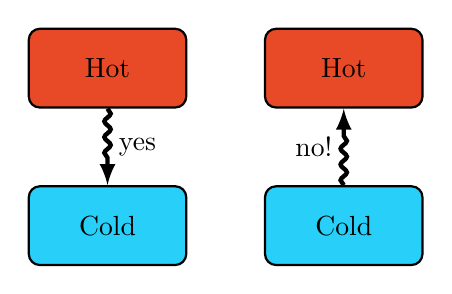
\begin{tikzpicture}[auto,every text node part/.style={align=center}]

	\node (TH1) at (0,0) [draw, rectangle, fill=Dorange, rounded corners, minimum width=2cm, minimum height = 1cm,  thick] {Hot};
	\node (TC1) at ($(TH1) + (0,-2)$) [draw, rectangle, fill=Dteal, rounded corners, minimum width=2cm, minimum height = 1cm,  thick] {Cold};
	\draw [ultra thick, -latex,decorate,decoration={snake,amplitude=.4mm,segment length=2mm, post length=9pt}] (TH1.south) -- (TC1.north) node[midway]{yes} ;

	\node (TH2) at  ($(TH1) + (3,0)$)  [draw, rectangle, fill=Dorange, rounded corners, minimum width=2cm, minimum height = 1cm, thick] {Hot};
	\node (TC2) at ($(TH2) + (0,-2)$) [draw, rectangle, fill=Dteal, rounded corners, minimum width=2cm, minimum height = 1cm, thick] {Cold};
	\draw [ultra thick, -latex,decorate,decoration={snake,amplitude=.4mm,segment length=2mm, post length=9pt}] (TC2.north) -- (TH2.south) node[midway]{no!} ;

\end{tikzpicture}\end{center}
\caption{Schematic illustration of the Clausius Statement of the Second Law.}\label{fig:Clausius}
\end{figure}


\subsubsection{Expansion} A gas trapped in a rigid chamber will fill this container's volume.  If this chamber is to expand, the gas will \emph{spontaneously} expand to fill the entire chamber

\begin{figure}[h]
\begin{center}
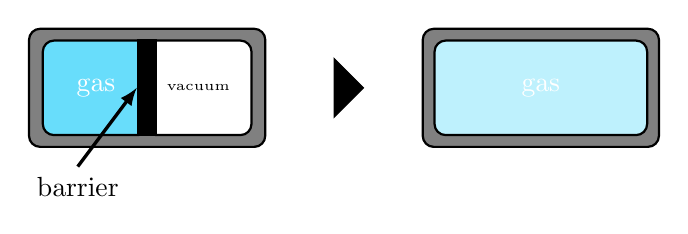
\begin{tikzpicture}[auto,every text node part/.style={align=center}]

	\node (C1) at (0,0) [draw, rectangle, fill=gray, rounded corners, minimum width=3cm, minimum height = 1.5cm, thick] {};
	\node (C1in) at (C1) [draw, rectangle, fill=Dteal!70, rounded corners, minimum width=1.35cm, minimum height = 1.2cm, thick,xshift=-0.65cm,text=white] {gas};
	\node (C1vac) at (C1) [draw, rectangle, fill=white, rounded corners, minimum width=1.35cm, minimum height = 1.2cm, thick,xshift=0.65cm] {\tiny{vacuum}};
	\node (barrier) at (C1) [draw, rectangle, fill=black, minimum width=0.05cm, minimum height = 1.2cm, thick] {};
	\draw [latex-,very thick] (barrier.west) -- ($(barrier.west) - (0.75,1)$) node[below] {barrier};
	
	\node [single arrow, draw, fill=black, minimum height=0.25cm, outer sep=0pt] at  ($(C1)+(2.5,0)$) {};
	

	\node (C2) at ($(C1)+(5,0)$) [draw, rectangle, fill=gray, rounded corners, minimum width=3cm, minimum height = 1.5cm, thick] {};
	\node (C2in) at (C2) [draw, rectangle, fill=Dteal!30, rounded corners, minimum width=2.7cm, minimum height = 1.2cm, thick,text=white] {gas};

\end{tikzpicture}\end{center}
\caption{Spontaneous expansion of a gas.}\label{fig:GasExpansion}
\end{figure}

A closed system energy balance on the chamber illustrates that the gas experiences no energy change, \emph{i.e.}, because no heat transfer occurred and no work was done on or by the system.
\begin{align*}
\Delta U = U_{\text{after}} - U_{\text{before}} &= Q - W \\
U_{\text{after}} - U_{\text{before}} &= 0 
\end{align*}
Though the energy has not changed, the energy has spread out, or dispersed, within the chamber, meaning there are 
more ways for the energy to exist in the chamber, or that the gas has more \textbf{microstates} available to it. 
\subsubsection{Directionality}
\begin{figure}[h]
\begin{center}
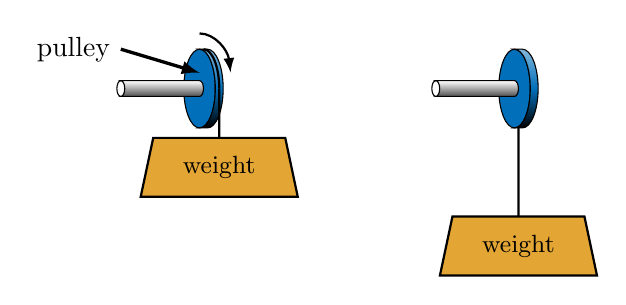
\begin{tikzpicture}[auto,every text node part/.style={align=center}]


	\draw[fill=Dlblue](0,0) circle (-0.2 and 0.5);
	\draw[top color=Dlblue!50,bottom color=black,middle color=Dlblue] (0.1,0.5) arc (90:270:-0.2 and 0.5) -- ++(-0.1,0) arc (-90:-270:-0.2 and 0.5) -- cycle;
	\draw[top color=white,bottom color=black!70] (0,1mm) arc (90:-90:0.5mm and 1mm)--++(-1cm,0) arc (-90:90:0.5mm and 1mm)-- cycle;
	%\draw[top color=white,bottom color=black!70] (0,3mm) arc (90:270:1.5mm and 3mm)--++(3cm,0) arc (-90:-270:1.5mm and 3mm)-- cycle;
	\draw (-1cm,1mm) arc (90:270:0.5mm and 1mm);

	\node (weight) at (0.25,-1) [draw, fill =Dlorange, trapezium, minimum width=2cm, trapezium angle =78,  outer sep=0pt, thick] {\small{weight}};
	\draw[thick] (0.05,0.5) arc (90:180:-0.2 and 0.5);
	\draw[thick] (0.25,0) -- (weight.north);
	
	\draw[thick, -latex] (0,0.7) arc (90:170:-0.4 and 0.6);
	
	\draw[very thick, -latex] (-1cm,0.5cm) node[left]{pulley}-- (0,0.2cm);
	

	\draw[fill=Dlblue](4,0) circle (-0.2 and 0.5);
	\draw[top color=Dlblue!50,bottom color=black,middle color=Dlblue] (4.1,0.5) arc (90:270:-0.2 and 0.5) -- ++(-0.1,0) arc (-90:-270:-0.2 and 0.5) -- cycle;
	\draw[top color=white,bottom color=black!70] (4,1mm) arc (90:-90:0.5mm and 1mm)--++(-1cm,0) arc (-90:90:0.5mm and 1mm)-- cycle;
	%\draw[top color=white,bottom color=black!70] (0,3mm) arc (90:270:1.5mm and 3mm)--++(3cm,0) arc (-90:-270:1.5mm and 3mm)-- cycle;
	\draw (3cm,1mm) arc (90:270:0.5mm and 1mm);

	\node (weight) at (4.05,-2) [draw, fill =Dlorange, trapezium, minimum width=2cm, trapezium angle =78,  outer sep=0pt, thick] {\small{weight}};
	\draw[thick] (4.05,-0.5) -- (weight.north);

\end{tikzpicture}\end{center}
\caption{Spontaneous lowering of a weight on a pulley.}\label{fig:WeightLower}
\end{figure}
From observations of spontaneous processes, it is suggested that the second law restricts the directionality of processes. Spontaneous processes such as falling objects (Fig.~\ref{fig:WeightLower}) and cooling frying pans are encountered every day. Spontaneous processes are \textbf{irreversible}, meaning that after they occur, the system and all parts of its surroundings cannot be exactly restored to their respective initial states. Auxiliary processes that can return the system to its initial state (\emph{i.e.}, raise the object or heat the pan), also change the state of the surroundings. These experiences suggest a directionality to processes that is formalized by the second law of thermodynamics. 



\subsection{Kelvin-Planck Statement of the Second Law}
\paragraph{Statement:}It is impossible for any system to operate in a thermodynamic cycle and deliver a net amount of energy by work to its surroundings while receiving energy by heat transfer from a single thermal reservoir.
\vspace{12pt}

\noindent\textbf{Any hypothetical system that violates either the first or the second laws of thermodynamics cannot be.}

\subsection{Clausius Inequality}
The \textbf{Clausius inequality}, a collary of the second law, states that for \emph{any} thermodynamic cycle
\begin{equation}\label{eq:ClausiusIneq}
\oint \left(\frac{\delta Q}{T}\right)_b \leq 0
\end{equation}
where $\delta Q$ is the heat transfer across some part of the system boundary for some portion of the cycle, and $T$ is the absolute temperature at that part of the system boundary, of which we are reminded by the subscript `b'.
\subsubsection{Reversible Process}
\begin{itemize}
    \item A cycle is reversible when the Clausius inequality becomes equality.
    \item In a \textbf{reversible process}, the system and all parts of its surroundings can be exactly restored to their respective initial states after the process has taken place.
    \item Such processes cannot occur in reality.   
\end{itemize}
\subsubsection{Internally Reversible Cycles}
Internally reversible processes contain no irreversibilities within the system, but can interact with surroundings that include irreversibilities. Thus the validity of the equality holds, even in surroundings where irreversibilities occur. 

\subsection{What is Entropy?}
For a reversible processes, the integral of $\delta Q/T$ is \emph{path independent}, and this thermodynamic property is called \textbf{entropy}.
\begin{equation}
S_2 - S_1 = \left(\int_1^2 \frac{\delta Q}{T}\right)_{\text{int rev}}.
\end{equation}
\begin{itemize}
    \item Entropy $S$ is the measure of energy dispersal as a function of temperature.
    \item \textbf{Entropy is a state function}, with the state being determined by any two intensive thermodynamic properties.
    \item  An entropy change for an \emph{incompressible substance} depends only on temperature.
\end{itemize}

\subsubsection{Differential form of the closed system energy balance}
The differential form of the closed system energy balance for an internally reversible process on a simple, compressible system can be written as,
\begin{equation}\label{eq:fund}
du = T ds - pdv
\end{equation}
\subsubsection{Specific Entropy of an Ideal Gas}
For an \emph{ideal gas} with a given, \textbf{constant specific heat $c_v$}, its change in specific entropy from a state $1$ to a state $2$ is given by the expression
\begin{equation}
s_2 - s_1 = c_v\ln\frac{T_2}{T_1}+ R \ln\frac{v_2}{v_1}
\end{equation}
where $R$ is the gas constant and $v$ is the specific volume. 
\vspace{14pt}

\noindent For an \emph{ideal gas} with a given, \textbf{constant specific heat $c_p$}, its change in specific entropy is given by the expression.
\begin{equation}
s_2 - s_1 = c_p\ln\frac{T_2}{T_1}- R \ln\frac{p_2}{p_1}.
\end{equation}

\subsubsection{Differential form of the enthalpy equation}
This differential equation of enthalpy and Eqn.~\eqref{eq:fund} are both known as \textbf{fundamental equations} of thermodynamics and relate thermodynamic properties between states. We use these expressions and the ideal gas as a model substance to gain some physical insight about entropy. 
\begin{equation}
dh = Tds + v dp.
\end{equation}
%%%%%%%%%%%%%%%%%%%%%%%%%%%%%%%%%%%%%%%%%%%%%%%%%%%%%%%%%%%%%%%%%%%%%%%%%%%%%%%%%%%%%%%%%%%%%%%%%%%%%%%%%%%%%%%%%%
\subsection{Entropy Balance}
The closed system entropy statement of the second law derives from the Clausius Inequality which in turn derives from the Kelvin-Planck statement. As we have shown, this statement is
\begin{equation}\label{eq:Centropy1}
S_2 - S_1 = \left(\int_1^2 \frac{\delta Q}{T}\right)_{\text{b}} +\sigma 
\end{equation}
where $\sigma$ represents the \textbf{entropy produced in the system} due to the irreversibilities (Fig.~\ref{fig:EntropyBal}) in the process and the `b' indicates that the heat is transferred across a boundary having temperature $T_b$. To satisfy the second law, \underline{$\sigma \geq 0$}. Entropy production $\sigma$ only equals zero when a process is reversible. 

\begin{center}[h]
\begin{tikzpicture}[auto,every text node part/.style={align=center},
	declare function={
        		curve(\x) = \x^2 + 0.875*\x+0.36;
		curve2(\x) = (1.7-0.3)/(0.8+0.8)*(\x+0.8)+0.3;
  	}
	]
	\node (ref2) at ($ (ref) + (5,0)$) [draw=none, coordinate] {};
	\begin{axis} [at={(ref2)},xmin=-1, ymin=0, xmax=1, ymax = 2, samples = 50, 
			ytick=\empty, yticklabels={}, ylabel style={rotate=-90},
			xtick=\empty, xticklabels={},
			width = 6cm, height=6cm, axis y line = left, axis x line = bottom,
			domain = -0.8:0.8, fill between/on layer={axis background}]
		
		\addplot[name path=g, black, very thick,-stealth] {curve(x)};
		\addplot[name path=h, black, very thick,stealth-,dashed] {curve2(x)};
		\addplot[draw=none,decoration={text along path, text align=center, text={irreversible process},}, postaction={decorate}]  {curve(x)+0.1};%mark options={decoration={name=none}} <- not needed here, but might be sometimes.
		\addplot[draw=none,decoration={text along path, text align=center, text={reversible process},}, postaction={decorate}]  {curve2(x)+0.1};
		\addplot [only marks] coordinates {
		(-0.8, {curve(-0.8)})
		(0.8, {curve(0.8)})
		};
		\node [above, color=black] at (axis cs:-0.8, {curve(-0.8)}) {\circled{$1$}};
		\node [above, color=black] at (axis cs:0.8, {curve(0.8)}) {\circled{$2$}};
	\end{axis}
\end{tikzpicture}\end{center}\label{fig:EntropyBal}
\paragraph{Expanded Derivation:}
\begin{equation}
\left(\int_1^2 \frac{\delta Q}{T}\right)_{\text{b}} + \left(\int_2^1 \frac{\delta Q}{T}\right)_{\text{b}} &\leq 0
\end{equation}
\begin{equation}
\left(\int_1^2 \frac{\delta Q}{T}\right)_{\text{b}} + S_1 - S_2 & = -\sigma 
\end{equation}
\begin{equation}
S_2 - S_1 &= \left(\int_1^2 \frac{\delta Q}{T}\right)_{\text{b}} +\sigma \label{eq:EntropyBal}
\end{equation}
\subsubsection{Entropy Balance and multiple heat transfer events}
When boundary temperature is constant, and multiple, distinct heat transfers occur, Eqn.~\eqref{eq:Centropy1} becomes
\begin{equation}\label{eq:EntropyBalance}
S_2 - S_1 = \sum_i \frac{Q_i}{T_{\text{b},i}} +\sigma. 
\end{equation}

\subsubsection{Rate of Change of Entropy}
In the absence of mass flow, the rate of change of the entropy in a system is derived as 
\begin{align}
\frac{d}{dt}\left(S - S_0\right) &= \frac{d}{dt}\left( \sum_i \frac{Q_i}{T_{\text{b},i}} +\sigma \right) \\
\frac{dS}{dt} &=\sum_i \frac{\dot{Q}_i}{T_{\text{b},i}} +\dot{\sigma}.
\end{align}


\subsubsection{Microstates}
The sets of possible configurations of the molecules are known as \textbf{microstates} and a state has a higher entropy when there are more microstates available to it.

\noindent When adding mass to a system (as shown via
a two-dimensional gas of two particles in a volume, which is then doubled as shown at the top of Fig.~\ref{fig:Indistinguishable}), 
\begin{itemize}
    \item If the added particles are identical to the original particles (indistinguishable).  Therefore, the two `microstates' at the lower left are exactly the same even if the particles switch places, and this counts as only one microstate. 
    \item On the other hand, for distinguishable particles, the two microstates are different. More microstates means higher entropy, thus when combining dissimilar materials there is a so-called \emph{entropy of mixing}. (\emph{This course does not include entropy of mixing.})
    \item The addition of identical substances requires no \emph{entropy of mixing} and therefore entropy of the new system increases in direct proportion to its increase in mass.
\end{itemize}

\begin{figure}[h]
\begin{center}
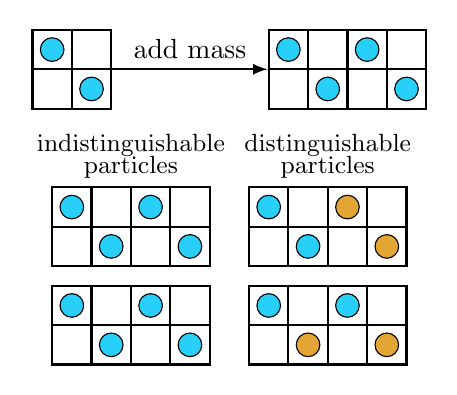
\begin{tikzpicture}[auto,every text node part/.style={align=center}]
	\node (box1) at (0,0) [draw, rectangle, minimum width=1cm, minimum height=1cm,thick]{};
	\draw [fill=Dteal] ($(box1)+(-0.25,0.25)$) circle (0.15cm);
	\draw [fill=Dteal] ($(box1)+(0.25,-0.25)$) circle (0.15cm);
	\draw [thick] (box1.north) -- (box1.south);
	\draw [thick] (box1.west) -- (box1.east);
	
	\node (box2) at ($(box1)+(3,0)$) [draw, rectangle, minimum width=1cm, minimum height=1cm,thick]{};
	\draw [fill=Dteal] ($(box2)+(-0.25,0.25)$) circle (0.15cm);
	\draw [fill=Dteal] ($(box2)+(0.25,-0.25)$) circle (0.15cm);
	\draw [thick] (box2.north) -- (box2.south);
	\draw [thick] (box2.west) -- (box2.east);
	\node (box) at ($(box2)+(1,0)$) [draw, rectangle, minimum width=1cm, minimum height=1cm,thick]{};
	\draw [fill=Dteal] ($(box)+(-0.25,0.25)$) circle (0.15cm);
	\draw [fill=Dteal] ($(box)+(0.25,-0.25)$) circle (0.15cm);
	\draw [thick] (box.north) -- (box.south);
	\draw [thick] (box.west) -- (box.east);
	
	\draw [-latex,thick] (box1.east) -- (box2.west) node[midway]{add mass};

	\node (box) at ($(box1)+(0.25,-2)$) [draw, rectangle, minimum width=1cm, minimum height=1cm,thick]{};
	\draw [fill=Dteal] ($(box)+(-0.25,0.25)$) circle (0.15cm);
	\draw [fill=Dteal] ($(box)+(0.25,-0.25)$) circle (0.15cm);
	\draw [thick] (box.north) -- (box.south);
	\draw [thick] (box.west) -- (box.east);
		
	\node(label1) at  ($(box)+(0.5,0.9)$) [draw=none]{\small{indistinguishable}\\[-4pt]\small{particles}};
	
	\node (box) at ($(box)+(1,0)$) [draw, rectangle, minimum width=1cm, minimum height=1cm,thick]{};
	\draw [fill=Dteal] ($(box)+(-0.25,0.25)$) circle (0.15cm);
	\draw [fill=Dteal] ($(box)+(0.25,-0.25)$) circle (0.15cm);
	\draw [thick] (box.north) -- (box.south);
	\draw [thick] (box.west) -- (box.east);


	\node (box) at ($(box1)+(0.25,-3.25)$) [draw, rectangle, minimum width=1cm, minimum height=1cm,thick]{};
	\draw [fill=Dteal] ($(box)+(-0.25,0.25)$) circle (0.15cm);
	\draw [fill=Dteal] ($(box)+(0.25,-0.25)$) circle (0.15cm);
	\draw [thick] (box.north) -- (box.south);
	\draw [thick] (box.west) -- (box.east);
	\node (box) at ($(box)+(1,0)$) [draw, rectangle, minimum width=1cm, minimum height=1cm,thick]{};
	\draw [fill=Dteal] ($(box)+(-0.25,0.25)$) circle (0.15cm);
	\draw [fill=Dteal] ($(box)+(0.25,-0.25)$) circle (0.15cm);
	\draw [thick] (box.north) -- (box.south);
	\draw [thick] (box.west) -- (box.east);

	\node (box) at ($(box1)+(2.75,-2)$) [draw, rectangle, minimum width=1cm, minimum height=1cm,thick]{};
	\draw [fill=Dteal] ($(box)+(-0.25,0.25)$) circle (0.15cm);
	\draw [fill=Dteal] ($(box)+(0.25,-0.25)$) circle (0.15cm);
	\draw [thick] (box.north) -- (box.south);
	\draw [thick] (box.west) -- (box.east);

	\node(label1) at  ($(box)+(0.5,0.9)$) [draw=none]{\small{distinguishable}\\[-4pt]\small{particles}};
	
	\node (box) at ($(box)+(1,0)$) [draw, rectangle, minimum width=1cm, minimum height=1cm,thick]{};
	\draw [fill=Dlorange] ($(box)+(-0.25,0.25)$) circle (0.15cm);
	\draw [fill=Dlorange] ($(box)+(0.25,-0.25)$) circle (0.15cm);
	\draw [thick] (box.north) -- (box.south);
	\draw [thick] (box.west) -- (box.east);

	\node (box) at ($(box1)+(2.75,-3.25)$) [draw, rectangle, minimum width=1cm, minimum height=1cm,thick]{};
	\draw [fill=Dteal] ($(box)+(-0.25,0.25)$) circle (0.15cm);
	\draw [fill=Dlorange] ($(box)+(0.25,-0.25)$) circle (0.15cm);
	\draw [thick] (box.north) -- (box.south);
	\draw [thick] (box.west) -- (box.east);
	\node (box) at ($(box)+(1,0)$) [draw, rectangle, minimum width=1cm, minimum height=1cm,thick]{};
	\draw [fill=Dteal] ($(box)+(-0.25,0.25)$) circle (0.15cm);
	\draw [fill=Dlorange] ($(box)+(0.25,-0.25)$) circle (0.15cm);
	\draw [thick] (box.north) -- (box.south);
	\draw [thick] (box.west) -- (box.east);
	
\end{tikzpicture}\end{center}
\caption{An illustration of the effect of distinguishable versus indistinguishable particles on microstates and therefore on system entropy.}\label{fig:Indistinguishable}
\end{figure}


\subsubsection{Principal of Superposition}
Entropy added to a system thus follows a \textbf{principal of superposition} meaning that the total system entropy, $S$, is the sum of the sub-system entropies.
\begin{equation}
S = \sum_i m_is_i,
\end{equation}
where each subsystem `$i$' of mass $m_i$ has specific entropy $s_i$ relative to some universal reference state.
\subsubsection{Open System Entropy Rate Balance}
It follows that for an \emph{open system} involving no mixing of substances, the entropy rate balance is simply
\begin{equation}\label{eq:EntropyRateBalance}
\frac{dS}{dt} =\sum_i \frac{\dot{Q}_i}{T_{\text{b},i}} + \sum_{\text{in}} \dot{m}_{\text{in}}s_{\text{in}} - \sum_{\text{out}} \dot{m}_{\text{out}}s_{\text{out}} + \dot{\sigma} .
\end{equation}




\section{Power Cycles}
Much of the power that we use in our daily lives is produced through cycles operating with a working fluid.

%%%%%%%%%%%%%%%%%%%%%%%%%%%%%%%%%%%%%%%%%%%%%%%%%%%%%%%%%%%%%%%%%%%%%%%%%%%%%%%%%%%%%%%%%%%%%%%%%%%%%%%%%%%%%%%%%%%%%%%%%%%%%%%%%%%%
\subsection{Carnot cycle}
A \textbf{Carnot cycle} is defined as an ideal gas, undergoing a 4-step, reversible, closed thermodynamic cycle. Imagine that an ideal gas contained within a piston-cylinder undergoes the series of processes depicted in Fig.~\ref{fig:CarnotCycle} below, with the gas starting in state $1$ before progressing to states $2$, $3$, $4$, and then returning to state $1$ to complete a cycle. 
%%%%%%%%%%%%%%%%%%%%%%%%%%%%%%%%%%%%%%%%%%%%%%%%%%%%%%%%%%%%%%%%%%%%%%%%%%%%%%%%%%%%%%%%%%%%%%%%%%%%%%%%%%%%%%%%%%
\begin{figure}[h]
\begin{center}
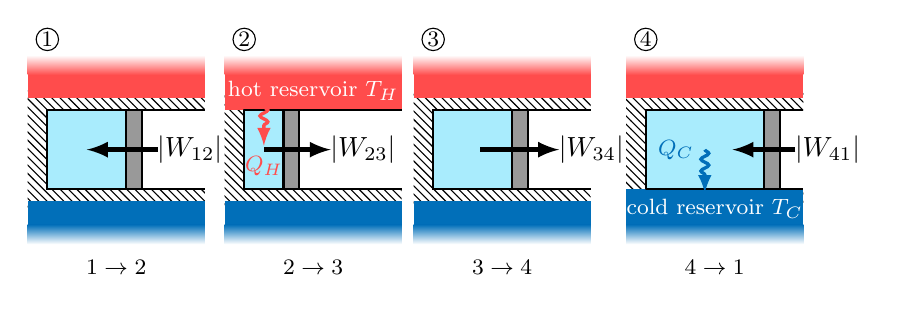
\begin{tikzpicture}[auto,every text node part/.style={align=center},>=latex']
%pistons
% State1 cylinder
	\node (ref) at (0,0) [draw=none, coordinate] {};
	\draw [ thick, join=round] ($ (ref) + (2,1)$) --  ($ (ref) + (0,1) $) -- (ref) -- ($ (ref) + (2,0)$);
	\draw (ref) [ thick, fill=Mteal] rectangle($ (ref) + (1,1)$); % define rectangle by lower left and upper right points
	\draw ($ (ref) + (1,0)$) [ thick, fill=gray!80] rectangle($ (ref) + (1.2,1)$); % define rectangle by lower left and upper right points
	\draw ($ (ref) + (0,1.9)$) node[circle, inner sep=0.5pt, draw]  {\footnotesize $1$};
	\draw [ultra thick, -latex] ($ (ref) + (1.4,0.5)$)  node[right, xshift=-0.15cm] {$|W_{12}|$} -- ($ (ref) + (0.5,0.5)$);
	\draw [ draw=none, pattern=north west lines, pattern color=black] (ref) -- ($ (ref) + (0,1)$) -- ($ (ref) + (2,1)$) -- ($ (ref) + (2,1.25)$) -- ($ (ref) + (-0.25,1.25)$) -- ($ (ref) + (-0.25,-0.25)$) -- ($ (ref) + (2,-0.25)$) -- ($ (ref) + (2,0)$) -- cycle; % insulated region
	\draw ($ (ref) + (-0.25,1.15)$) [ draw= none, fill=red!70] rectangle($ (ref) + (2,1.5)$); % define rectangle by lower left and upper right points, hot reservoir
	\draw ($ (ref) + (-0.25,1.45)$) [ draw= none, top color=white, bottom color=red!70] rectangle($ (ref) + (2,1.7)$); % define rectangle by lower left and upper right points, hot reservoir
	\draw ($ (ref) + (-0.25,-0.5)$) [ draw= none, fill=Dlblue] rectangle($ (ref) + (2,-0.15)$); % define rectangle by lower left and upper right points, cold reservoir
	\draw ($ (ref) + (-0.25,-0.45)$) [ draw= none, top color=Dlblue, bottom color=white] rectangle($ (ref) + (2,-0.7)$); % define rectangle by lower left and upper right points, hot reservoir
	\draw ($ (ref) + (0.875,-1)$) node[draw = none]  {\footnotesize $1 \to 2$};

% State2 cylinder
	\node (ref2) at  ($ (ref) + (2.5,0)$)  [draw=none, coordinate] {};
	\draw (ref2) [ thick, fill=Mteal] rectangle($ (ref2) + (0.5,1)$); % define rectangle by lower left and upper right points
	\draw ($ (ref2) + (0.5,0)$) [ thick, fill=gray!80] rectangle($ (ref2) + (0.7,1)$); % define rectangle by lower left and upper right points
	\draw ($ (ref2) + (0,1.9)$) node[circle, inner sep=0.5pt, draw]  {\footnotesize $2$};
	\draw [ultra thick, latex-] ($ (ref2) + (1.1,0.5)$)  node[right, xshift=-0.15cm] {$|W_{23}|$} -- ($ (ref2) + (0.25,0.5)$);
	\draw [ draw=none, pattern=north west lines, pattern color=black] (ref2) -- ($ (ref2) + (0,1)$) -- ($ (ref2) + (2,1)$) -- ($ (ref2) + (2,1.25)$) -- ($ (ref2) + (-0.25,1.25)$) -- ($ (ref2) + (-0.25,-0.25)$) -- ($ (ref2) + (2,-0.25)$) -- ($ (ref2) + (2,0)$) -- cycle; % insulated region
	\draw ($ (ref2) + (-0.25,1)$) [ draw= none, fill=red!70] rectangle($ (ref2) + (2,1.5)$); % define rectangle by lower left and upper right points, hot reservoir
	\draw ($ (ref2) + (-0.25,1.45)$) [ draw= none, top color=white, bottom color=red!70] rectangle($ (ref2) + (2,1.7)$); % define rectangle by lower left and upper right points, hot reservoir
	\draw ($ (ref2) + (-0.25,-0.5)$) [ draw= none, fill=Dlblue] rectangle($ (ref2) + (2,-0.15)$); % define rectangle by lower left and upper right points, cold reservoir
	\draw ($ (ref2) + (-0.25,-0.45)$) [ draw= none, top color=Dlblue, bottom color=white] rectangle($ (ref2) + (2,-0.7)$); % define rectangle by lower left and upper right points, hot reservoir
	\draw ($ (ref2) + (0.875,-1)$) node[draw = none]  {\footnotesize $2 \to 3$};
	\draw [ thick, join=round] ($ (ref2) + (2,1)$) --  ($ (ref2) + (0,1) $) -- (ref2) -- ($ (ref2) + (2,0)$);
	\draw[-latex,decorate,decoration={snake,amplitude=.5mm,segment length=1.5mm ,post length=6pt}, very thick, draw=red!70, color=red!70] ($ (ref2) + (0.25,1.05)$) -- ($ (ref2) + (0.25,0.55)$)  node[below, text=red!70] {\footnotesize $Q_H$} ;
	\draw ($ (ref2) + (0.875,1.25)$) node[draw = none, text=white]  {\footnotesize hot reservoir $T_H$};
	%\draw ($ (ref2) + (-0.25,1.8)$) node[draw = none, text=red!20]  {\footnotesize $T_H$};
	
% State3 cylinder
	\node (ref3) at  ($ (ref2) + (2.4,0)$)  [draw=none, coordinate] {};
	\draw [ thick, join=round] ($ (ref3) + (2,1)$) --  ($ (ref3) + (0,1) $) -- (ref3) -- ($ (ref3) + (2,0)$);
	\draw (ref3) [ thick, fill=Mteal] rectangle($ (ref3) + (1,1)$); % define rectangle by lower left and upper right points
	\draw ($ (ref3) + (1,0)$) [ thick, fill=gray!80] rectangle($ (ref3) + (1.2,1)$); % define rectangle by lower left and upper right points
	\draw ($ (ref3) + (0,1.9)$) node[circle, inner sep=0.5pt, draw]  {\footnotesize $3$};
	\draw [ultra thick, latex-] ($ (ref3) + (1.6,0.5)$)  node[right,xshift=-0.15cm] {$|W_{34}|$} -- ($ (ref3) + (0.6,0.5)$);
	\draw [ draw=none, pattern=north west lines, pattern color=black] (ref3) -- ($ (ref3) + (0,1)$) -- ($ (ref3) + (2,1)$) -- ($ (ref3) + (2,1.25)$) -- ($ (ref3) + (-0.25,1.25)$) -- ($ (ref3) + (-0.25,-0.25)$) -- ($ (ref3) + (2,-0.25)$) -- ($ (ref3) + (2,0)$) -- cycle; % insulated region
	\draw ($ (ref3) + (-0.25,1.15)$) [ draw= none, fill=red!70] rectangle($ (ref3) + (2,1.5)$); % define rectangle by lower left and upper right points, hot reservoir
	\draw ($ (ref3) + (-0.25,1.45)$) [ draw= none, top color=white, bottom color=red!70] rectangle($ (ref3) + (2,1.7)$); % define rectangle by lower left and upper right points, hot reservoir
	\draw ($ (ref3) + (-0.25,-0.5)$) [ draw= none, fill=Dlblue] rectangle($ (ref3) + (2,-0.15)$); % define rectangle by lower left and upper right points, cold reservoir
	\draw ($ (ref3) + (-0.25,-0.45)$) [ draw= none, top color=Dlblue, bottom color=white] rectangle($ (ref3) + (2,-0.7)$); % define rectangle by lower left and upper right points, hot reservoir
	\draw ($ (ref3) + (0.875,-1)$) node[draw = none]  {\footnotesize $3 \to 4$};
	
% State4 cylinder
	\node (ref4) at  ($ (ref3) + (2.7,0)$)  [draw=none, coordinate] {};
	\draw (ref4) [ thick, fill=Mteal] rectangle($ (ref4) + (1.5,1)$); % define rectangle by lower left and upper right points
	\draw ($ (ref4) + (1.5,0)$) [ thick, fill=gray!80] rectangle($ (ref4) + (1.7,1)$); % define rectangle by lower left and upper right points
	\draw ($ (ref4) + (0,1.9)$) node[circle, inner sep=0.5pt, draw]  {\footnotesize $4$};
	\draw [ultra thick, -latex] ($ (ref4) + (1.9,0.5)$)  node[right,xshift=-0.15cm] {$|W_{41}|$} -- ($ (ref4) + (1.1,0.5)$);
	\draw [ draw=none, pattern=north west lines, pattern color=black] (ref4) -- ($ (ref4) + (0,1)$) -- ($ (ref4) + (2,1)$) -- ($ (ref4) + (2,1.25)$) -- ($ (ref4) + (-0.25,1.25)$) -- ($ (ref4) + (-0.25,-0.25)$) -- ($ (ref4) + (2,-0.25)$) -- ($ (ref4) + (2,0)$) -- cycle; % insulated region
	\draw ($ (ref4) + (-0.25,1.15)$) [ draw= none, fill=red!70] rectangle($ (ref4) + (2,1.5)$); % define rectangle by lower left and upper right points, hot reservoir
	\draw ($ (ref4) + (-0.25,1.45)$) [ draw= none, top color=white, bottom color=red!70] rectangle($ (ref4) + (2,1.7)$); % define rectangle by lower left and upper right points, hot reservoir
	\draw ($ (ref4) + (-0.25,-0.5)$) [ draw= none, fill=Dlblue] rectangle($ (ref4) + (2,0)$); % define rectangle by lower left and upper right points, cold reservoir
	\draw ($ (ref4) + (-0.25,-0.45)$) [ draw= none, top color=Dlblue, bottom color=white] rectangle($ (ref4) + (2,-0.7)$); % define rectangle by lower left and upper right points, hot reservoir
	\draw ($ (ref4) + (0.875,-1)$) node[draw = none]  {\footnotesize $4 \to 1$};
	\draw [ thick, join=round] ($ (ref4) + (2,1)$) --  ($ (ref4) + (0,1) $) -- (ref4) -- ($ (ref4) + (2,0)$);
	\draw[-latex,decorate,decoration={snake,amplitude=.5mm,segment length=1.5mm ,post length=6pt}, very thick, draw=Dlblue, color=Dlblue] ($ (ref4) + (0.75,0.5)$) node[left, text=Dlblue] {\footnotesize $Q_C$} -- ($ (ref4) + (0.75,-0.05)$);
	\draw ($ (ref4) + (0.875,-0.25)$) node[draw = none, text=white]  {\footnotesize cold reservoir $T_C$};

\end{tikzpicture}\end{center}
\caption{A schematic of a piston-cylinder executing a Carnot cycle between hot and cold thermal reservoirs. }\label{fig:CarnotCycle}
\end{figure}
%%%%%%%%%%%%%%%%%%%%%%%%%%%%%%%%%%%%%%%%%%%%%%%%%%%%%%%%%%%%%%%%%%%%%%%%%%%%%%%%%%%%%%%%%%%%%%%%%%%%%%%%%%%%%%%%%%

During the cycle, the system contacts sequentially a hot reservoir and a cold reservoir at temperatures $T_H$ and $T_C$, respectively. While in contact with a thermal reservoir, the system remains at the temperature of the thermal reservoir. In between reservoir contacts, the system is insulated and no heat transfer occurs. Each process \textbf{quasi-static}, and \textbf{reversible}. In this idealized cycle, heat transfers in and out of the system despite the fact that there is no temperature difference to drive heat flow. Such hypothetical heat flow is reversible because an infinitesimal increase in the reservoir temperature relative to the system will cause heat to flow into the system, or vice versa for an infinitesimal decrease in the reservoir temperature. This idealized cycle is known as a Carnot cycle. 

\paragraph{Reversible process:} In a reversible process, the direction can be reversed at any point by an infinitesimal change in external conditions. 

\paragraph{Quasi-static process:} A process that occurs at an infinitesimally slow rate so that the system is in a thermodynamic equilibrium at all times.

\subsubsection{Carnot Cycle Steps}

In processes $2 \to 3$ and $3 \to 4$, work is done by the gas. Figure~\ref{fig:PVwork1} illustrates two potential, monotonic processes corresponding to positive work, or work done by the gas. On the left, pressure is higher in state $b$ than state $a$. On the right, pressure is higher in state $a$ than state $b$. $V_b > V_a$ in both cases. When illustrating the magnitude of the work to be determined, the arrow is drawn out of the system as shown in state $1$. 


\begin{figure}[h]
\begin{center}
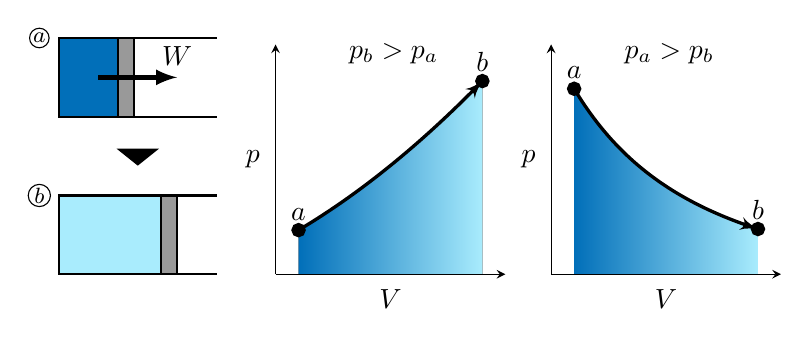
\begin{tikzpicture}[auto,>=latex',
	declare function={
        		curve1(\x) = \x^2;
		curve2(\x) = 1/(\x^2);
  	}
	]

% upper cylinder
	\node (ref) at (0,0) [draw=none, coordinate] {};
	\draw [ thick, join=round] ($ (ref) + (2,1)$) -- ($ (ref) + (0,1) $) -- (ref) -- ($ (ref) + (2,0)$);
	\draw (ref) [ thick, fill=Dlblue] rectangle($ (ref) + (0.75,1)$); % define rectangle by lower left and upper right points
	\draw ($ (ref) + (0.75,0)$) [ thick, fill=gray!80] rectangle($ (ref) + (0.95,1)$); % define rectangle by lower left and upper right points
	\draw ($ (ref) + (-0.25,1)$) node[circle, inner sep=0.5pt, draw]  {\footnotesize $a$};
	\draw [ultra thick, -latex] ($ (ref) + (0.5,0.5)$)  -- ($ (ref) + (1.5,0.5)$) node[above] {$W$};
% lower cylinder
	\node (ref2) at ($ (ref) - (0,2)$) [draw=none, coordinate] {};
	\draw [ thick, join=round] ($ (ref2) + (2,1)$) -- ($ (ref2) + (0,1) $) -- (ref2) -- ($ (ref2) + (2,0)$);
	\draw (ref2) [ thick, fill=Mteal] rectangle($ (ref2) + (1.3,1)$); % define rectangle by lower left and upper right points
	\draw ($ (ref2) + (1.3,0)$) [ thick, fill=gray!80] rectangle($ (ref2) + (1.5,1)$);  % define rectangle by lower left and upper right points
	\draw ($ (ref2) + (-0.25,1)$) node[circle, inner sep=0.5pt, draw]  {\footnotesize $b$};
	% arrow between
	\node [isosceles triangle, draw, fill=black, isosceles triangle stretches, minimum height=0.2cm, minimum width=0.5cm, shape border rotate=-90, inner sep=0pt] at ($ (ref) + (1,-0.5)$) {};
	
% left plot
	\node (refp1) at ($ (ref) + (2.75,-2)$) [draw=none, coordinate] {};
	\begin{axis} [at={(refp1)},xmin=1, ymin=0.5, xmax=2, ymax = 4.2, samples = 50, 
			ytick=\empty, yticklabels={}, ylabel style={rotate=-90},
			xtick=\empty, xticklabels={},
			ylabel={$p$}, xlabel={$V$},
			width = 4.5cm, height=4.5cm, axis y line = left, axis x line = bottom,
			domain = 1.1:1.9, fill between/on layer={axis background}]
		
		\addplot[name path=f, black, very thick,->] {curve1(x)}; % Curve
		\path[name path=ax] (axis cs:1, 0.5) -- (axis cs:2, 0.5); % Axis base to shade to
		\addplot [left color = Dlblue, right color = Mteal] % Add shaded region
		fill between [
			of = f and ax,
			soft clip={domain=1.1:1.9},
		];
		\addplot [only marks, very thick] coordinates { % Add end points
		(1.1, {curve1(1.1)})
		(1.9, {curve1(1.9)})
		};
		\node [above, color=black] at (axis cs:1.1, {curve1(1.1)}) {$a$};
		\node [above, color=black] at (axis cs:1.9, {curve1(1.9)}) {$b$};
		
	\end{axis}
	\draw ($ (refp1) + (1.5,2.8)$) node[draw=none] {$p_b>p_a$};

% right plot
	\node (refp2) at ($ (refp1) + (3.5,0)$) [draw=none, coordinate] {};
	\begin{axis} [at={(refp2)},xmin=1, ymin=0.1, xmax=2, ymax = 1, samples = 50, 
			ytick=\empty, yticklabels={}, ylabel style={rotate=-90},
			xtick=\empty, xticklabels={},
			ylabel={$p$}, xlabel={$V$},
			width = 4.5cm, height=4.5cm, axis y line = left, axis x line = bottom,
			domain = 1.1:1.9, fill between/on layer={axis background}]
		
		\addplot[name path=g, black, very thick,->] {curve2(x)};
		\path[name path=ax2] (axis cs:1, 0.1) -- (axis cs:2, 0.1);
		\addplot [left color = Dlblue, right color = Mteal]
		fill between [
			of = g and ax2,
			soft clip={domain=1.1:1.9},
		];
		\addplot [only marks, very thick] coordinates {
		(1.1, {curve2(1.1)})
		(1.9, {curve2(1.9)})
		};
		\node [above, color=black] at (axis cs:1.1, {curve2(1.1)}) {$a$};
		\node [above, color=black] at (axis cs:1.9, {curve2(1.9)}) {$b$};
	\end{axis}
	\draw ($ (refp2) + (1.5,2.8)$) node[draw=none] {$p_a>p_b$};

\end{tikzpicture}
\end{center}
\caption{Work done by the gas}\label{fig:PVwork1}
\end{figure}


In processes $1 \to 2$ and $4 \to 1$, work is done on the gas. Figure~\ref{fig:PVwork1} illustrates two potential, monotonic processes corresponding to positive work, or work done by the gas. On the left, pressure is higher in state $b$ than state $a$. On the right, pressure is higher in state $a$ than state $b$. $V_a > V_b$ in both cases as shown in Figure~\ref{fig:PVwork2}. Recall the expression for $pV$ work,
\begin{equation}
W = \int_{V_a}^{V_b} p(V) dV,
\end{equation}
noting that work for these processes is negative as indicated by the right-to-left process curve arrow in each of the $pV$ diagrams. When illustrating the magnitude of the work to be determined, the arrow is drawn into the system as shown in state $a$ (Fig.~\ref{fig:PVwork2}). 

\begin{figure}[h]
\begin{center}
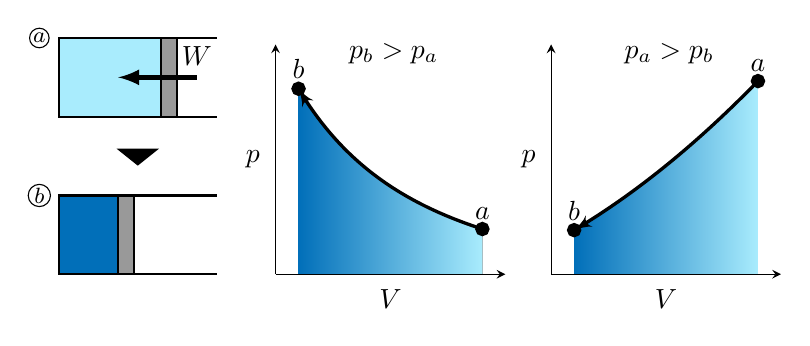
\begin{tikzpicture}[auto,>=latex',
	declare function={
        		curve1(\x) = 1/(\x^2);
		curve2(\x) = \x^2;
  	}
	]

% upper cylinder
	\node (ref) at (0,0) [draw=none, coordinate] {};
	\draw [ thick, join=round] ($ (ref) + (2,1)$) -- ($ (ref) + (0,1) $) -- (ref) -- ($ (ref) + (2,0)$);
	\draw (ref) [ thick, fill=Mteal] rectangle($ (ref) + (1.3,1)$); % define rectangle by lower left and upper right points
	\draw ($ (ref) + (1.3,0)$) [ thick, fill=gray!80] rectangle($ (ref) + (1.5,1)$);  % define rectangle by lower left and upper right points
	\draw ($ (ref) + (-0.25,1)$) node[circle, inner sep=0.5pt, draw]  {\footnotesize $a$};
	\draw [ultra thick, latex-] ($ (ref) + (0.75,0.5)$)  -- ($ (ref) + (1.75,0.5)$) node[above] {$W$};
% lower cylinder
	\node (ref2) at ($ (ref) - (0,2)$) [draw=none, coordinate] {};
	\draw [ thick, join=round] ($ (ref2) + (2,1)$) -- ($ (ref2) + (0,1) $) -- (ref2) -- ($ (ref2) + (2,0)$);
	\draw (ref2) [ thick, fill=Dlblue] rectangle($ (ref2) + (0.75,1)$); % define rectangle by lower left and upper right points
	\draw ($ (ref2) + (0.75,0)$) [ thick, fill=gray!80] rectangle($ (ref2) + (0.95,1)$); % define rectangle by lower left and upper right points
	\draw ($ (ref2) + (-0.25,1)$) node[circle, inner sep=0.5pt, draw]  {\footnotesize $b$};
	% arrow between
	\node [isosceles triangle, draw, fill=black, isosceles triangle stretches, minimum height=0.2cm, minimum width=0.5cm, shape border rotate=-90, inner sep=0pt] at ($ (ref) + (1,-0.5)$) {};
	
% left plot
	\node (refp1) at ($ (ref) + (2.75,-2)$) [draw=none, coordinate] {};
	\begin{axis} [at={(refp1)},xmin=1, ymin=0.1, xmax=2, ymax = 1, samples = 50, 
			ytick=\empty, yticklabels={}, ylabel style={rotate=-90},
			xtick=\empty, xticklabels={},
			ylabel={$p$}, xlabel={$V$},
			width = 4.5cm, height=4.5cm, axis y line = left, axis x line = bottom,
			domain = 1.1:1.9, fill between/on layer={axis background}]
		
		\addplot[name path=f, black, very thick,<-] {curve1(x)}; % Curve
		\path[name path=ax] (axis cs:1, 0.1) -- (axis cs:2, 0.1); % Axis base to shade to
		\addplot [left color = Dlblue, right color = Mteal] % Add shaded region
		fill between [
			of = f and ax,
			soft clip={domain=1.1:1.9},
		];
		\addplot [only marks, very thick] coordinates { % Add end points
		(1.1, {curve1(1.1)})
		(1.9, {curve1(1.9)})
		};
		\node [above, color=black] at (axis cs:1.1, {curve1(1.1)}) {$b$};
		\node [above, color=black] at (axis cs:1.9, {curve1(1.9)}) {$a$};
		
	\end{axis}
	\draw ($ (refp1) + (1.5,2.8)$) node[draw=none] {$p_b>p_a$};

% right plot
	\node (refp2) at ($ (refp1) + (3.5,0)$) [draw=none, coordinate] {};
	\begin{axis} [at={(refp2)},xmin=1, ymin=0.5, xmax=2, ymax = 4.2, samples = 50, 
			ytick=\empty, yticklabels={}, ylabel style={rotate=-90},
			xtick=\empty, xticklabels={},
			ylabel={$p$}, xlabel={$V$},
			width = 4.5cm, height=4.5cm, axis y line = left, axis x line = bottom,
			domain = 1.1:1.9, fill between/on layer={axis background}]
		
		\addplot[name path=g, black, very thick,<-] {curve2(x)};
		\path[name path=ax2] (axis cs:1, 0.5) -- (axis cs:2, 0.5);
		\addplot [left color = Dlblue, right color = Mteal]
		fill between [
			of = g and ax2,
			soft clip={domain=1.1:1.9},
		];
		\addplot [only marks, very thick] coordinates {
		(1.1, {curve2(1.1)})
		(1.9, {curve2(1.9)})
		};
		\node [above, color=black] at (axis cs:1.1, {curve2(1.1)}) {$b$};
		\node [above, color=black] at (axis cs:1.9, {curve2(1.9)}) {$a$};
	\end{axis}
	\draw ($ (refp2) + (1.5,2.8)$) node[draw=none] {$p_a>p_b$};

\end{tikzpicture}
\end{center}
\caption{Work done on the gas}\label{fig:PVwork2}
\end{figure}

To plot the processes that make up the cycle in Fig.~\ref{fig:CarnotCycle}, we first observe that processes $2 \to 3$ and $4 \to 1$ are \textbf{isothermal}, meaning the temperature of the working fluid is constant during the process. Given that the working fluid is an ideal gas, $pV = mRT$ and therefore 
\begin{equation}\label{eq:IG_eos2}
p = \frac{mR}{V} T
\end{equation}
where $m$ is the mass of gas and $R$ is the gas constant. An isothermal process at $T_H$ or $T_C$, the temperature of the hot and cold reservoirs, must therefore fall on the dashed lines in Fig.~\ref{fig:CarnotpV}. These lines are known as \textbf{isotherms}. 

\begin{figure}[h]
\begin{center}
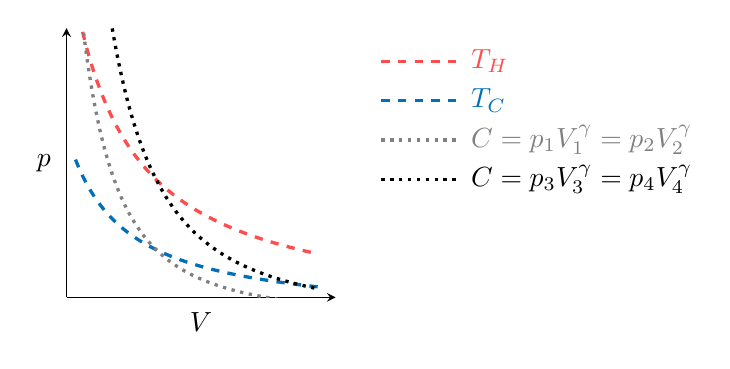
\begin{tikzpicture}[auto,>=latex',
	declare function={
        		curveTH(\x) = 1/(\x);
		curveTC(\x) = 0.5/(\x);
		curveR(\x) = 0.8/(\x^(2));
		curveL(\x) = 0.4/(\x^(2));
  	}
	]

% plot
	\node (ref) at (0,0) [draw=none, coordinate] {};
	\begin{axis} [at={(ref)}, xmin=0.3, ymin=0.2, xmax=1.8, ymax = 2.6, samples = 100, 
			ytick=\empty, yticklabels={}, ylabel style={rotate=-90},
			xtick=\empty, xticklabels={},
			ylabel={$p$}, xlabel={$V$},
			width = 5cm, height=5cm, axis y line = left, axis x line = bottom,
			domain = 0.35:1.7, fill between/on layer={axis background}]
		
		\addplot[red!70, very thick, dashed] {curveTH(x)};
		\addplot[Dlblue, very thick,dashed] {curveTC(x)};
		\addplot[black!50, very thick,dotted] {curveL(x)};
		\addplot[black, very thick,dotted] {curveR(x)};

	\end{axis}
	\node (refL) at ($ (ref) + (4,3)$) [draw=none, coordinate] {};
	\draw [dashed, very thick, red!70] ($ (refL) + (0,0)$) -- ($ (refL) + (1cm,0)$) node[right, draw=none] {$T_H$};
	\draw [dashed, very thick, Dlblue] ($ (refL) + (0,-0.5cm)$) -- ($ (refL) + (1cm,-0.5cm)$) node[right, draw=none] {$T_C$};
	\draw [dotted, very thick, black!50] ($ (refL) + (0,-1cm)$) -- ($ (refL) + (1cm,-1cm)$) node[right, draw=none] {$C = p_1V_1^{\gamma} = p_2V_2^{\gamma}$};
	\draw [dotted, very thick, black] ($ (refL) + (0,-1.5cm)$) -- ($ (refL) + (1cm,-1.5cm)$) node[right, draw=none] {$C = p_3V_3^{\gamma} = p_4V_4^{\gamma}$};

\end{tikzpicture}
\end{center}
\caption{$pV$ curves for ideal gas expansion and compression in a Carnot cycle.}\label{fig:CarnotpV}
\end{figure}

Processes $1 \to 2$ and $3 \to 4$ are \textbf{adiabatic}, meaning that during the process no heat transfer occurs. We will show later in the class that the adiabatic, reversible expansion or compression of an ideal gas must obey the relation
\begin{equation}\label{eq:polytropic}
pV^{\gamma}=C
\end{equation}
where $\gamma$ and $C$ are constants and $\gamma > 1$. Therefore these processes must fall on a curve defined by
\begin{equation}
\label{eq:Pexpression}
p(V)=\frac{C}{V^{\gamma}},
\end{equation}
illustrated for two values of $C$ by the dash-dot lines in Fig.~\ref{fig:CarnotpV}. 

Combining the $p(V)$ relations for the ideal gas expansion and compression with the directionality of the work shown in Figs.~\ref{fig:PVwork1} and \ref{fig:PVwork2}, we can plot a Carnot cycle for an ideal gas on a $pV$ diagram as shown in Fig.~\ref{fig:CarnotpVcycle}. 

\begin{figure}[h]
\begin{center}
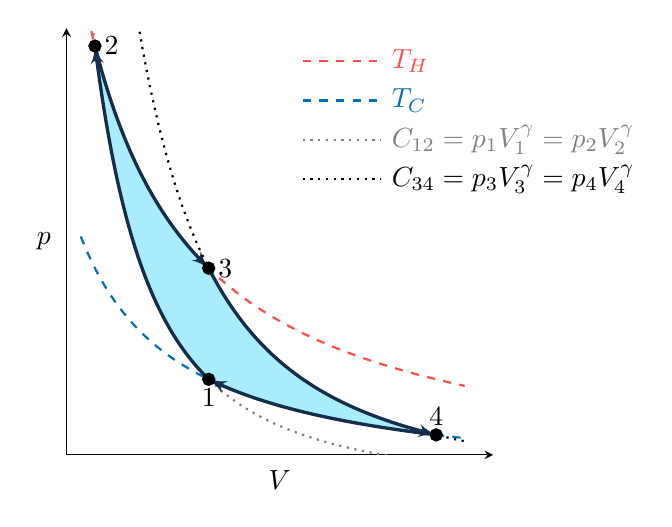
\begin{tikzpicture}[auto,>=latex',
	declare function={
        		curveTH(\x) = 1/(\x);
		curveTC(\x) = 0.5/(\x);
		curveR(\x) = 0.8/(\x^(2));
		curveL(\x) = 0.4/(\x^(2));
  	}
	]

% plot
	\node (ref) at (0,0) [draw=none, coordinate] {};
	\begin{axis} [at={(ref)}, xmin=0.3, ymin=0.2, xmax=1.8, ymax = 2.6, samples = 100, 
			ytick=\empty, yticklabels={}, ylabel style={rotate=-90},
			xtick=\empty, xticklabels={},
			ylabel={$p$}, xlabel={$V$},
			width = 7cm, height=7cm, axis y line = left, axis x line = bottom,
			domain = 0.35:1.7, fill between/on layer={axis background}]
		
		\addplot[red!70,  thick, dashed] {curveTH(x)};
		\addplot[Dlblue,  thick,dashed] {curveTC(x)};
		\addplot[black!50,  thick,dotted] {curveL(x)};
		\addplot[black,  thick,dotted] {curveR(x)};
		\addplot[name path=hot, Ddblue, very thick, domain=0.4:0.8, ->] {curveTH(x)};
		\addplot[name path=cold, Ddblue, very thick, domain={0.4/0.5}:{0.8/0.5}, <-] {curveTC(x)};
		\addplot[name path=left, Ddblue, very thick, domain=0.4:{0.4/0.5}, <-] {curveL(x)};
		\addplot[name path=right, Ddblue, very thick, domain=0.8:{0.8/0.5}, ->] {curveR(x)};
		\addplot [Mteal, draw=Mteal]
		fill between [
			of = hot and left,
			soft clip={domain=0.4:0.8},
		];
		\addplot [Mteal]
		fill between [
			of = right and cold,
			soft clip={domain=0.8:{0.8/0.5}},
		];
		\addplot [only marks, thick] coordinates {
		({0.4/0.5}, {curveTC(0.4/0.5)})
		(0.4, {curveTH(0.4)})
		(0.8, {curveTH(0.8)})
		({0.8/0.5}, {curveTC(0.8/0.5)})
		};
		\node [below, color=black] at (axis cs:{0.4/0.5}, {curveTC(0.4/0.5)}) {$1$};
		\node [right, color=black] at (axis cs:{0.4}, {curveTH(0.4)}) {$2$};
		\node [right, color=black] at (axis cs:{0.8}, {curveTH(0.8)}) {$3$};		
		\node [above, color=black] at (axis cs:{0.8/0.5}, {curveTC(0.8/0.5)}) {$4$};
	\end{axis}
	\node (refL) at ($ (ref) + (3,5)$) [draw=none, coordinate] {};
	\draw [dashed,  thick, red!70] ($ (refL) + (0,0)$) -- ($ (refL) + (1cm,0)$) node[right, draw=none] {$T_H$};
	\draw [dashed,  thick, Dlblue] ($ (refL) + (0,-0.5cm)$) -- ($ (refL) + (1cm,-0.5cm)$) node[right, draw=none] {$T_C$};
	\draw [dotted,  thick, black!50] ($ (refL) + (0,-1cm)$) -- ($ (refL) + (1cm,-1cm)$) node[right, draw=none] {$C_{12} = p_1V_1^{\gamma} = p_2V_2^{\gamma}$};
	\draw [dotted,  thick, black] ($ (refL) + (0,-1.5cm)$) -- ($ (refL) + (1cm,-1.5cm)$) node[right, draw=none] {$C_{34} = p_3V_3^{\gamma} = p_4V_4^{\gamma}$};

\end{tikzpicture}
\end{center}
\caption{A $pV$ diagram for an ideal gas undergoing a Carnot cycle as depicted in Fig.~\ref{fig:CarnotCycle}.}\label{fig:CarnotpVcycle}
\end{figure}

The work done by the cycle $W$ is positive and equal to the shaded area in Fig.~\ref{fig:CarnotpVcycle}, where the net work is described as the sum of the work done during each of the processes,
\begin{equation}
W= W_{12} + W_{23} + W_{34} + W_{41}
\end{equation}

\subsubsection{Isothermal Processes}
For isothermal processes $2 \to 3$ and $4 \to 1$ the work is determined by the $p(V)$ relation in Eqn~\eqref{eq:IG_eos2}
which yields
\begin{equation}
W_{23} =mRT_H\ln\left(\frac{V_3}{V_2}\right) \,\,\text{ and }\,\, W_{41} = mRT_C\ln\left(\frac{V_1}{V_4}\right)
\end{equation}
Because temperature is not changing and the fluid is an ideal gas, the change in internal energy for these processes is zero. An energy balance on the gas for each of these processes yields
\begin{equation}\label{eq:QH}
Q_{23} = Q_{H} = W_{23} = mRT_H\ln\left(\frac{V_3}{V_2}\right) 
\end{equation}
where $Q_H$ refers to the heat transferred into the system from the hot reservoir and 
\begin{equation}\label{eq:QC}
Q_{41} = - Q_{C} = W_{41} = mRT_C\ln\left(\frac{V_1}{V_4}\right)
\end{equation}
where $Q_C$ refers to the heat transferred from the system to the cold reservoir. 
\subsubsection{Adiabatic Processes}
For adiabatic, reversible processes $1 \to 2$ and $3 \to 4$ the work is given by
\begin{equation}
W_{12} = \int_{V_1}^{V_2} \frac{C_{12}}{V^{\gamma}} dV \text{ and } W_{34} = \int_{V_3}^{V_4} \frac{C_{34}}{V^{\gamma}} dV
\end{equation}
which, when integrated yield
\begin{equation}
\begin{gathered}
W_{12} =\frac{-C_{12}}{\gamma-1}\left(\frac{1}{V_2^{\gamma-1}} - \frac{1}{V_1^{\gamma-1}}\right) \\
\text{ and } \\
 W_{34} = \frac{-C_{34}}{\gamma-1}\left(\frac{1}{V_4^{\gamma-1}} - \frac{1}{V_3^{\gamma-1}}\right) 
\end{gathered}
\end{equation}
Multiplying both sides of the relation in Eqn.~\eqref{eq:polytropic} by $1/V^{\gamma-1}$ and using the resulting relation, $pV = C/V^{\gamma-1}$, combined with the ideal gas equation of state, we can express the work in the adiabatic, reversible processes as
\begin{equation}
W_{12} =\frac{mR(T_C - T_H)}{\gamma - 1}  \,\,\text{ and }\,\, W_{34} = \frac{mR(T_H - T_C)}{\gamma - 1}
\end{equation}
illustrating that the work in these two processes are equal in magnitude but opposite in sign. 
It is interesting to determine the relationship between volume and temperature in the end states of processes $1 \to 2$ and $3 \to 4$ for the ideal gas. For an infinitesimal change in internal energy $dU$ no heat flow occurs, but an infinitesimal amount of $pV$ work is done, $\delta W = p dV$. We write this infinitesimal form of the energy balance as
\begin{equation} 
d U = \cancelto{0}{\delta Q} - \delta W = -p dV
\end{equation}
For an ideal gas, $dU/dT = mc_v$ and $p = mRT/V$ so that
\begin{equation}
c_v dT = -\frac{RT}{V} dV
\end{equation}
Separating the volume $V$ and temperature $T$ and integrating, between states $1$ and $2$ yields
\begin{equation} \label{eq:VT12}
\int_{T_C}^{T_H} \frac{c_v}{RT} dT =  \ln\left(\frac{V_1}{V_2}\right).
\end{equation}
Integrating between states $4$ and $3$ yields 
\begin{equation} \label{eq:VT43}
\int_{T_C}^{T_H} \frac{c_v}{RT} dT = \ln\left(\frac{V_4}{V_3}\right).
\end{equation}
The left hand side of both Eqns.~\eqref{eq:VT12} and \eqref{eq:VT43} are equal so that 
\begin{equation}
\ln\left(\frac{V_1}{V_2}\right) = \ln\left(\frac{V_4}{V_3}\right).
\end{equation}
or equivalently\sidenote{ $\ln(x/y) = \ln x - \ln y$.}
\begin{equation} \label{eq:V1234}
\ln\left(\frac{V_1}{V_4}\right) = \ln\left(\frac{V_2}{V_3}\right).
\end{equation}
Recalling the results from the energy balances on the isothermal processes (Eqns.~\eqref{eq:QH} and \eqref{eq:QC}) we can show that the ratio of the heat influx $Q_H$ to heat loss $Q_C$ is
\begin{equation}
\frac{Q_H}{Q_C} = \frac{T_H\ln\left(\frac{V_3}{V_2}\right) }{T_H\ln\left(\frac{V_4}{V_1}\right)}
\end{equation}
Applying Eqn.~\eqref{eq:V1234}, which defines the relationship between the states before and after the adiabatic processes, we obtain
\begin{equation} \label{eq:HeatTemp}
\frac{Q_H}{Q_C} = \frac{T_H}{T_C}
\end{equation}
for an ideal gas undergoing a Carnot cycle. 
\subsubsection{Internal Energy Balance of the System}
The total change in the internal energy of the Carnot cycle $\Delta U$ can alternately be determined by an energy balance on the cycle
\begin{align}
\Delta U&= Q - W \label{eq:Ebalance} \\
&= Q_H - Q_C - W_{12} - \underbrace{W_{23}}_{=Q_H} - \underbrace{W_{34}}_{=-W_{12}} - \underbrace{W_{41}}_{=-Q_C} \label{eq:Ebaldetailed} \\
&= 0
\end{align}
Thus the Carnot cycle is consistent with the energy change for a cycle in general.
\subsubsection{Thermal Efficiency}
This Carnot cycle turns heat input $Q_H$ into work output $W$. The thermal efficiency $\eta$ for such a \textbf{heat engine} is given by 
\begin{equation}
\eta = \frac{\text{net work output}}{\text{heat input}} = \frac{W}{Q_H}
\end{equation}
Combining $\Delta U = 0$ for a cycle, the expression for the energy balance on the cycle (Eqns.~\eqref{eq:Ebalance} and \eqref{eq:Ebaldetailed}), and the temperature-heat transfer relationship found in Eqn.~\eqref{eq:HeatTemp} yields
\begin{equation}
\eta = \frac{Q_H - Q_C}{Q_H} = 1-\frac{T_C}{T_H}.
\end{equation}
A Carnot cycle produces the maximum possible efficiency for any heat engine. The efficiency can only approach $1$ (equivalent to 100\%) when either $T_C \to 0$ or $T_H \to \infty$, neither of which is physically attainable. 
%%%%%%%%%%%%%%%%%%%%%%%%%%%%%%%%%%%%%%%%%%%%%%%%%%%%%%%%%%%%%%%%%%%%%%%%%%%%%%%%%%%%%%%%%%%%%%%%%%%%%%%%%%%%%%%%%%%%%%%%%%%%%%%%%%%
\subsection{A Rankine Cycle}
The Rankine cycle is the basis for steam-electric power plants, which produce nearly 90\% of all electricity worldwide.  This cycle includes two isentropic processes, and utilizes isobaric heat transfers. 
\begin{figure}[h]
\begin{center}
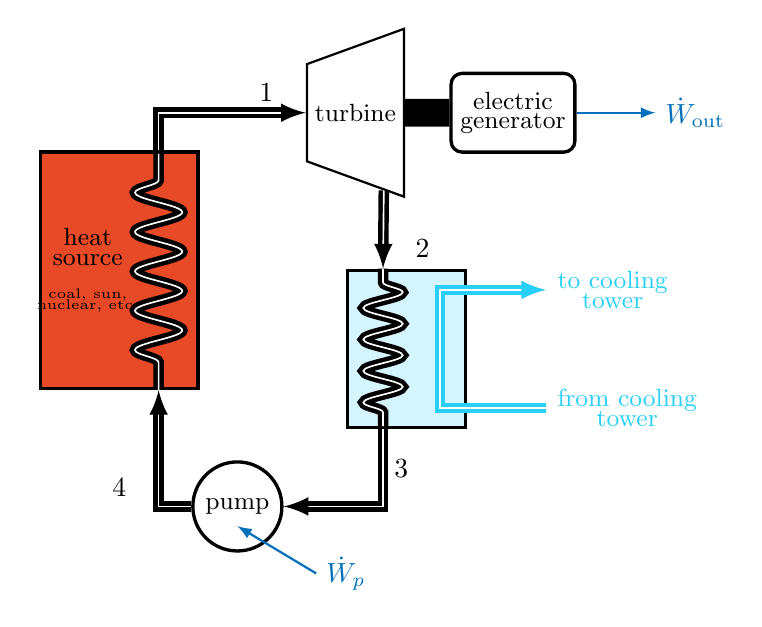
\begin{tikzpicture}[auto,every text node part/.style={align=center}]

	\node (hexIN) [draw, fill = Dorange, rectangle, minimum width = 2cm, minimum height = 3cm, very thick]{};
	\node (hexLabel) at (hexIN) [draw=none,color=black,xshift=-0.4cm] {\small{heat}\\[-5pt]\small{source}\\ \tiny{coal, sun,}\\[-8pt] \tiny{nuclear, etc.}};
	\node (turbine) at ($(hexIN) + (2,4)$) [draw, very thick, trapezium,trapezium left angle=70,trapezium right angle=70,rotate=90,minimum width=0.75cm, minimum height=0.75cm, 
	text width=1cm, text height = 1cm, text depth = 0cm, text centered,thick,yshift=-1cm, xshift=-2cm] {};
	\node (turbineLabel) at (turbine) [draw=none] {\small{turbine}};
	\node (hexOUT) at ($(turbine) + (0.65,-3)$) [draw, fill=Dteal!20,rectangle, minimum width = 1.5cm, minimum height = 2cm, very thick]{};
	\node (pump) at ($(hexIN) + (1.5,-3)$) [draw, circle, minimum width=0.75cm, very thick] {\small{pump}};
	
	
	\node (electric) at ($(turbine) + (2,0)$) [draw,rectangle, minimum width = 1.5cm, minimum height = 1cm, very thick, rounded corners] {\small{electric} \\[-5pt] \small{generator}};
	
	% power
	\draw [line width=10pt] (turbine.south) -- (electric.west);
	\draw [thick,latex-,color=Dlblue] ($(pump)+(0,-0.25)$) -- ++(1,-0.6) node[right] {$\dot{W}_p$};
	\draw [thick,-latex,color=Dlblue] (electric.east) -- ++(1,0) node[right] {$\dot{W}_{\text{out}}$};	

	% working fluid flow
	\draw [-,ultra thick,double, decorate,decoration={snake,amplitude=3mm,segment length=5mm, post length=8pt, pre length=10pt}] ($(hexIN.south)+(0.5,0)$) node[above,xshift=-0.25cm]{}-- ++(0,3);
	\draw [-latex,ultra thick,double] ($(hexIN.north)+(0.5,0)$) |- (turbine.north)  node[above, xshift=-0.5cm]{\circled{1}};
	\draw [-latex,ultra thick,double] (turbine.200) -- ($(hexOUT.north)+(-0.3,0)$) node[above, xshift=0.5cm]{\circled{2}};
	\draw [-,ultra thick,double, decorate,decoration={snake,amplitude=2.5mm,segment length=4mm, post length=4pt, pre length=5pt}] ($(hexOUT.north)+(-0.3,0)$) node[above,xshift=-0.25cm]{}-- ++(0,-2);
	\draw [-latex,ultra thick,double] ($(hexOUT.south)+(-0.3,0)$) node[right, yshift=-0.5cm]{\circled{3}} |- (pump.east) ;
	\draw [-latex,ultra thick,double] (pump.west) -| ($(hexIN.south)+(0.5,0)$) node[above, xshift=-0.5cm, yshift=-1.5cm]{\circled{4}};
	
	% cooling fluid
	\draw [-latex, ultra thick, double,color=Dteal] ($(hexOUT.east)+(1,-0.75)$) node[right] {\small{from cooling}\\[-5pt] \small{tower}}-- ($(hexOUT.east)+(-0.35,-0.75)$) -- ($(hexOUT.east)+(-0.35,0.75)$) -- ($(hexOUT.east)+(1,0.75)$) node[right] {\small{to cooling}\\[-5pt] \small{tower}};


\end{tikzpicture}\end{center}
\caption{A schematic of a vapor power plant capable of undergoing a Rankine cycle.}\label{fig:IdealRankineCycle}
\end{figure}

An ideal Rankine cycle consists of the following internally reversible processes: 
\begin{itemize}
\item \textbf{Process $1\to 2$:} Isentropic expansion of the working fluid through the turbine from saturated vapor at state $1$ to the condenser pressure $p_2$.
\item \textbf{Process $2\to 3$:} Heat transfer from the working fluid as it flows at constant pressure $p_2 = p_3$ through the condenser, exiting as a saturated liquid at state $3$. 
\item \textbf{Process $3\to 4$:} Isentropic compression in the pump to state $4$ in the compressed liquid region of the phase diagram.
\item \textbf{Process $4\to 1$:} Heat transfer to the working fluid as it flows at constant pressure $p_4 = p_1$ through the boiler to complete the cycle. 
\end{itemize}


Instead, the condenser stream is taken to the saturated liquid state, so that only a compressed liquid must be pumped.\sidenote{Cavitation is less of an issue in the two phase fluid used in the turbine since the vapor bubbles that form nearer the saturated vapor portion of the vapor dome are less driven to collapse.} While state $4$ could be taken all the way to $T_{\text{sat}}(p_4 = p_1)$, this would also lead to practical difficulties since, to maintain an isothermal heat transfer, a large thermal reservoir would be required. Instead, the process from state $4$ to state $1$ follows an isobar as shown in the plot below. 

\begin{figure}
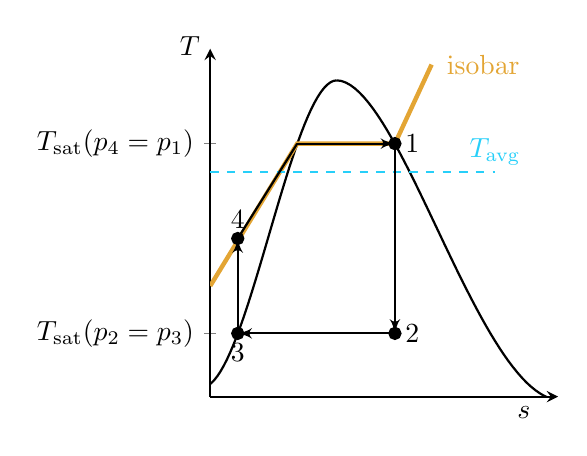
\begin{tikzpicture}[auto,>=latex',
	declare function={
        		curveL(\x) = -1.6*\x^2-0.25*x^3+10;
		curveR(\x) = -1*\x^2 + 0.3*x^2.5 + 10;
  	}
	]

	%%% Example isobar
	
	\node (ref) at (0,0) [draw=none, coordinate] {};
	\begin{axis} [at={(ref)},xmin=-4, ymin=0, xmax=7, ymax = 11, samples = 50, 
			ytick={2,8}, yticklabels={$T_{\text{sat}}(p_2 = p_3)$,$T_{\text{sat}}(p_4 = p_1)$},  ylabel style={rotate=-90},
			xtick=\empty, xticklabels=\empty,
			ylabel={$T$}, xlabel={$s$},
			width = 6cm, height=6cm, axis y line = left, axis x line = bottom,
			thick,ylabel style = {at={(axis description cs:0,0.95)},anchor=south east}, xlabel style = {at={(axis description cs:0.95,0)},anchor=north east}]

    	%L+V dome
            		\addplot[thick,domain=-5:0, name path=L] {curveL(x)};	
            		\path[name path=axL] (axis cs:-5, 0) -- (axis cs:0, 0);	
            		\addplot[thick,domain=0:7, name path=R] {curveR(x)};
            		\path[name path=axR] (axis cs:0, 0) -- (axis cs:14, 0);
	%isobar
			\addplot[ultra thick, mark=none,color=Dlorange] coordinates {(-4,3.5) (-1.25,8) (1.84,8) (3,10.5)} node[right,xshift=0.05cm]{isobar};
			
	% Tavg
			\addplot[thick,  dashed,color=Dteal] coordinates {(-4,7.1) (5,7.1)};
			\node [above, color=Dteal] at (axis cs:5, 7) {$T_{\text{avg}}$};
			
				% Cycle  		
			\addplot[thick,  ->] coordinates {(-1.25,8) (1.84,8)};
			\addplot[thick, ->] coordinates {(1.84,2) (-3.13,2)};
			\addplot[ thick,->] coordinates {(-3.13,2) (-3.13,5)};
			\addplot[thick] coordinates {(-3.13,5) (-1.25,8)};
			\addplot[thick, ->] coordinates {(1.84,8) (1.84,2)};
			\addplot [only marks, thick] coordinates {
			(-3.13,2) (-3.13,5)
			(1.84,2) (1.84,8)
			};

			
		\node [below, color=black] at (axis cs:-3.13, 2) {\circled{3}};
		\node [above, color=black] at (axis cs:-3.13, 5) {\circled{4}};
		\node [right, color=black] at (axis cs:1.84, 8) {\circled{1}};		
		\node [right, color=black] at (axis cs:1.84, 2) {\circled{2}};

	\end{axis}

\end{tikzpicture}
\caption{A $T$-$s$ diagram of an ideal Rankine cycle.}\label{fig:TsDiagramRankine}
\end{figure}

For reversible processes, the second law can be written as:
\begin{equation}
Q = \int T dS,
\end{equation}
 meaning that the area under the curve in a $T$-$s$ diagram corresponds to heat transferred to or from a system. Thus to approximate a Carnot cycle, an average temperature value at which the same heat transfer $Q_H$ occurs can be approximated on the diagram.
Since the Carnot cycle tells us that the maximum thermal efficiency of a power cycle is:
\begin{equation}
\eta = 1- Q_C/Q_H = 1-T_C/T_H
\end{equation} 
it is clear from Fig.~\ref{fig:TsDiagramRankine} that a hypothetical Carnot cycle with maximum operating temperature $T_H$ will always have a greater thermal efficiency than a Rankine cycle with the same maximum operating temperature since the \emph{average} operating temperature of the Rankine cycle is lower. 


\subsection{Otto Cycle}
The Otto cycle provides an approximation of the internal combustion engines that still make up the largest share of the transportation industry. 

An automotive internal combustion engine uses a reciprocating piston-cylinder action to produce work.  In a four-stroke engine
\begin{enumerate}
\item The intake valve is open and the piston makes an intake stroke to draw in a fresh charge, e.g., a combustible mixture of fuel and air. 
\item The intake valve closes and the piston undergoes a compression stroke that increases the pressure and temperature of the air within. At the end of the compression, combustion is induced, e.g., via a spark plug.
\item A power stroke follows as the gas mixture expands, doing work on the piston.
\item Finally, the exhaust valve is opened and burned gases are purged during an exhaust stroke.
\end{enumerate}

The Otto cycle simplifies this process by ignoring affects associated with the addition and removal of fuel. Instead it uses air, acting as an ideal gas, to provide insight into how such cycles can be optimized. The combustion itself is replaced by heat transfer and all processes are internally reversible. As a result, the Otto cycle consists of the following steps.
\begin{itemize}
\item \textbf{Process 1-2:} Isentropic compression of the air as the piston moves from bottom to top.
\item \textbf{Process 2-3:} Constant-volume heat transfer to the air from an external source while the piston is at the top. (Approximates fuel ignition and rapid burning.)
\item \textbf{Process 3-4:} Isentropic expansion (power stroke).
\item \textbf{Process 4-1:} Constant-volume process in which heat is rejected from the air while the piston is at the bottom.
\end{itemize}
Note that because it is operating within a piston cylinder, the states the processes operate between are the state of the air in the closed piston cylinder system. This is different from the Rankine cycle, in which the stream states change by going through processes facilitated by different thermodynamics devices. We will show in class that the thermal efficiency of an Otto cycle can be expressed entirely as a function of the compression ratio, $r$, defined as the ratio of the largest gas volume over the smallest $V_1/V_2$ according to:
\begin{equation}
\eta = 1-\frac{1}{r^{k-1}}
\end{equation}
and shows that engine efficiency can be increased by inducing a larger change in piston chamber volume. Of course, further practical considerations, such as the increased weight of such an engine, provide other design constraints. We only touch on a few of these design constraints, but in general thermodynamics provides many of the key principles through which energy systems can be optimized. 



\end{document}
